\documentclass[11pt]{whatsnote}
\usepackage{dsfont, wrapstuff, pgfpages}
\DeclareRobustCommand \identity {\mathds 1}
\coverset{
  title   = Condensed Matter Theory,
  author  = \ttfamily \textsc{Mingyu Xia},
  afill   = PhD @Westlake University,
  date    = November 2025,
  extinfo = {
\includegraphics[width = .1\paperwidth]{myhsia_seal}},
  head    = Hmolecule.png,
  clogo   = cat.pdf,
  llogos  = {mouse1.png, mouse2.png,
             mouse4.png, mouse5.png}
}

\begin{document}

\maketitle[purple!50!green]
\frontmatter
\tableofcontents
\mainmatter

\include{./context/0_Preparation.tex}
% !TeX root = ../main.tex

\chapter{}
% !TeX root = ../main.tex

\chapter{Free electron model of metals}

\section{Durde model (1900) for electrons in metals}

\section{Ohm's Law in macroscope}

\begin{equation}
  V = \int_a^b E \d x = Ed,~ V = IR
\end{equation}
Define current density $j = I/A$, therefore
\[
  Ed = jAR,~ E = \ab(\frac{RA}d) j
\]
then, we can define the conductivity $\sigma = 1/\rho$,
where $\rho = RA/d$ is the resistivity. So,
\begin{equation}
  \bm j = \sigma \bm E
\end{equation}

\section{Resistivity}

\begin{enumerate}
  \item Metals:
  \begin{itemize}
    \item Very conductive
    \item The resistivity increases with increasing temperature
  \end{itemize}
  \item Semiconductors
  \begin{itemize}
    \item Limited conductance
    \item The resistivity decreases with increasing temperature
  \end{itemize}
  \item Insulators: Very weak conductance
\end{enumerate}

\section{Summerfeld model (1920s) for electrons in metals}

\section{Drude model}

Without electric field:
\begin{itemize}
  \item Free electron moving randomly
  \item $\frac12 mv_\text{rms}^2 = \frac32 k_BT$, $v_\text{rms} = \qty{1.2e5}{\m/\s}$ at room temperature.
\end{itemize}

With elecric field, the drift velocity $v_\text d \ll v_\text{rms}$, $v_d \sim \qty{e-5}{\m/\s}$.
The definition of the drift velocity is $v_\text d = l/\tau$.

Let $\tau$ be the scattering time and $1/\tau$ be the scattering rate.
Consider in a time interval $\d t$, a fraction $\d t/\tau$ of th electrons are scattered, and their average velocity becomes zero.

\section{Classical Hall effet}

\section{Drude model with a magnetic field}

Consider Drude model with applied electric and magnetic fields:
\[
  m^* \dot{\bm v} = -e(\bm E + \bm v \times \bm B) - m^*\bm v/\tau
\]
In steady state, we have
\[
  \bm E = -\frac{m^*\bm v}{e\tau} - \bm v \times \bm B
\]
and we can rewritten it into 3 components:
\[
  \begin{aligned}
    & \frac{v_x}\tau - \omega_cv_y = -\frac em E_x\\
    & \frac{v_y}\tau + \omega_cv_x = -\frac em E_y\\
    & \frac{v_z}\tau = -\frac em E_z
  \end{aligned}
\]
then we arrive at
\[
  \begin{aligned}
    v_x & = -\frac{e\tau}{m(1 + \omega_c^2\tau^2)}(E_x + \omega_c\tau E_y)\\
    v_y & = -\frac{e\tau}{m(1 + \omega_c^2\tau^2)}(E_y - \omega_c\tau E_y)\\
    v_z & = -\frac{e\tau}m E_z
  \end{aligned}
\]
and we can write it into matrix form
\[
  \begin{pmatrix}
    v_x\\v_y\\v_z
  \end{pmatrix} =
  \hat\sigma
  \begin{pmatrix}
    E_x\\E_y\\E_z
  \end{pmatrix}
\]
or $\hat \rho = \sigma^{-1}$.

\section{Summerfeld Model}

\subsection{Electron wave}

Time-independent Schr\"odinger equation
\begin{equation}
  -\frac{\hbar^2}{2m} \nabla^2 \psi(\bm r) + U\psi(\bm r) = E\psi(\bm r)
\end{equation}
For a free electron: $U = 0$,
\[
  \nabla^2 \psi(\bm r) = -\frac{2mE}{\hbar^2}\psi(\bm r)
\]
The solution is a plane wave
\begin{equation}
  \psi(\bm r) = \frac1{\sqrt V}\upe^{\iu(k_xx+k_yy+k_zz)}
\end{equation}
Energy
\begin{equation}
  E = \frac{\hbar^2k^2}{2m} = \frac{\hbar^2(k_x^2 + k_y^2 + k_z^2)}{2m}
\end{equation}
apply the Born-von Karman periodic boundary conditions
\begin{equation}
  \begin{aligned}
    \psi(x + L_x,y,z) & = \psi(x,y,z)\\
    \psi(x,y + L_y,z) & = \psi(x,y,z)\\
    \psi(x,y,z + L_z) & = \psi(x,y,z)
  \end{aligned}
\end{equation}
States in $k$-space
\begin{equation}
  k_x = \frac{2\pi n_1}{L_x},~
  k_y = \frac{2\pi n_2}{L_y},~
  k_z = \frac{2\pi n_3}{L_z}
\end{equation}
with $n_i \in \mathbb Z$.
In each unit (3D grid) with size $d^3$: $\Delta d = \frac{2\pi}{L_x}[(x + 1) - (-x)]$.
The volume is $\frac{2\pi}{L_x} \cdot \frac{2\pi}{L_y} \cdot \frac{2\pi}{L_z}$, there are $2 \times V/(2\pi)^3$ quantum states per unit volume in $k$-space, while the density is $\frac2V = 2 \times \frac{1}{\ab(\prod_i\frac{2\pi}{L_i})}$.

One can simply think that the allowed states inside a sphere.
The volume of the sphere should be
\[
  V = \frac43\pi k_F^3
\]
while the density is
\[
  2 \times \frac1{(\frac{2\pi}{L})^3}
\]
then, the number of electrons in the sphere should be
\[
  N = 2 \times \frac{(4\pi/3)k_F^3}{(2\pi/L)^3} = \frac{k_F^3}{3\pi^2}V
\]
We define the \emph{Fermi wave vector}: $k_F = (3\pi^2 n)^{1/3}$, which we can compute it from the carrier density $n = N/V$.

\section{Bosons and Fermions at $T \neq 0$}

Bosoons:
\begin{equation}
  \bar n_i = \frac{g_i}{\exp}
\end{equation}

at $T = 0$,
\[
  f(E) =
  \begin{cases*}
    0, & for $E > E_f$\\
    1, & for $E < E_f$
  \end{cases*}
\]

\section{Fermi-Dirac Distribution}

\begin{equation}
  f(E) = \frac{1}{1 + \exp[(E - E_f)/k_BT]}
\end{equation}

\section{Density of states}

\[
  n(T) = \int f(E)g(E)\d E
\]
$g(E)$: how many states are allowed at energy $E$.

\begin{equation}
  g(E) = \frac1V \odv NE
\end{equation}
we cancalculate the total number
\begin{equation}
  N = \frac{k^3}{3\pi^2}V
\end{equation}
and
\begin{equation}
  E = \frac{\pi^2 k^2}{2n}
\end{equation}
Subsititute $E$ and $N$ into $g(E) = \frac1V\odv NE$, we can have
\begin{equation}
  g(E) = \frac{mk}{\hbar^2 \pi^2}
\end{equation}
which $k = \frac{\sqrt{2mE}}\hbar$.
\begin{enumext}[columns = 2]
  \item $g_{3D}(E) = \frac{m^*}{\pi^2 \hbar^3} \sqrt{2m^*E} \propto E^{1/2}$
  \item $g_{2D}(E) = \frac{m^*}{\pi \hbar^2} = \text{Const}$
  \item $g_{1D}(E) = \frac1{\pi \hbar} \sqrt{\frac{2m^*}{E}} \propto E^{-1/2}$
  \item $g_{0D}(E) = 2\delta(E)$
\end{enumext}
The total number of electron at $T > 0$ per volume
\[
  \frac NV = \int \underbrace{f(E)}_{probability} \cdot \underbrace{g(E) \d E}_{\text{can be occupied}}
\]
and the energy for the electrons at the Fermi energy level (internal energy) is
\begin{equation}
  \bar E = \int E f(E) g(E) \d E
\end{equation}
to calculate the velocity
\[
  v(E) = \int v(E) f(E) g(E) \d E, \qq{and}
  v(k) = \int v(k) f(k) g(k) \d k
\]
remember to add a $\frac{V}{(2\pi)^3}$ factor when calculate in $k$-space.
Then, the current density is
\begin{equation}
  \bm j = -ne\bm v = -2e \int \frac{\d^3 \bm k}{(2\pi)^3} f(\bm k) v(\bm k)
\end{equation}
Consider $\bm j = \sigma \bm E$,
when $\bm E = \bm 0$ then $\bm j = \bm 0$. Now, check it.
At zero field, for every occupied state $\bm k$, there is a state $-\bm k$ occupied with the same probability and the corresponding velocity is same but negative.

For the current density in an applied electric field,
\begin{equation}
  \bm j = -nev = -2e \int \frac{\d^3 \bm k}{(2\pi)^3} f\ab(\bm k + \frac{e\tau}{\hbar} \bm E) v(\bm k)
  = -2e \int \frac{\d^3 \bm k}{(2\pi)^3} f(\bm k) v\ab(\bm k - \frac{e\tau}{\hbar} \bm E)
\end{equation}
since $v(\bm k) = h\bm k/m$
\[
  \bm j = \frac{e^2\tau}{m} \ab[2\int \frac{\d^3\bm k}{(2\pi)^3} f(\bm k)] \bm E
= \frac{e^2\tau}{m} n \bm E = \sigma \bm E
\]
which $\sigma = ne\tau^2/m$ is the same as that in Drude mode.

\subsection{Heat capacity of an electron gas}

The change of internal energy when heated from $0K$ to $T > 0$
\begin{equation}
  \Delta U = U(T) - U(0) = \int - \int 
\end{equation}

\begin{itemize}
  \item At Mediate temperature: $T^3$
  \item At Low temperature: $T$
  \item At High temperature: Const
\end{itemize}

At low temperature, $f$ choose to be step function, and obviously,
$\pdv* fT$ will be like a $\delta$-function.

\subsection{Thermal transport}

\section{Limitation of Free electron gas model}

% !TeX root = ../main.tex

\chapter{Lattice Vibrations and Phonons}

\section{Specific head capacity in solids}

\begin{equation}
  m \odv[2]{u_n}t = \beta(u_{n+1} + u_{n-1} - 2u_n)
\end{equation}
should have wave-like solutions
\[
  u_n = A\upe^{\iu(\omega t - nak)}
\]
Subsititute it to the ODE, then we have the dispersion relation
\[
  \omega = 2\sqrt{\frac\beta m} \ab|\sin\ab(\frac{ka}{2})|
\]
\begin{itemize}
  \item The dispersion relation is perodic in $k$, \emph{with period $2\pi/a$}
  \item ...
\end{itemize}

$k = n \frac{2\pi}{Na}$
For a $n$-number of particles, we have n phonons, each phonon has a vibration, that is a $\omega$.

For small $ka$, $\omega \approx a \sqrt{\frac\beta m}|k|$.

$k \in [-\pi/a, \pi/a]$, $k \to k + 2\pi/a$

$\hbar \frac\pi a \frac23 \times 3 \to \frac{2\pi}{a}\hbar$

$-\frac23\hbar\frac\pi a \times 3$ $-\frac{2\pi}{a}\hbar + \frac{2\pi}{a} \hbar \times 2$

\subsection{A diatomic chain}

We have two kind of atoms, and keep the period. Using two kind of equations
\begin{gather}
  m \odv[2]{u_{2n}}t = \beta(u_{2n+1} + u_{2n-1} - 2u_{2n})\\
  M \odv[2]{u_{2n+1}}t = \beta(u_{2n+2} + u_{2n} - 2u_{2n+1})
\end{gather}
Similarly
\[
  u_{2n} = A\upe^{\iu (\omega t - 2nak)}
\]

\subsection{Gap}

For gap: at $k = \ab|\frac\pi{2a}|$, supposed $M > m$, we have
\[
  \omega_+^2 = \frac{2\beta}m > \omega_-^2 = \frac{2\beta}{M}
\]
when $m = M$, the gap equals to zero.
% !TeX root = ../main.tex

\chapter{Crystal Symmetry \& Crystal Structure}

\section{Crystal Symmetry}

\subsection{Inversion Symmetry}

\subsection{Rotoinversion Symmetry}

\section{Crystal Structure}

\begin{equation}
  \text{Crystal lattice} + \text{Basis} = \text{Crystal structure}
\end{equation}
Replace a every site (represent the symmetry of crystals) by basis (represent the compound of crystal: one / a group of atom / a molecule / a set of molecule): nvotif

Fourier transfor:
\begin{equation}
  \upe^{\iu\bm G\cdot\bm R} = 1,~
  A(k) = A(k) \upe^{\iu\bm k\cdot\bm R}
\end{equation}
then $\upe^{\iu\bm k\cdot\bm R} = 1$.

\begin{equation}
  \bm a_i \cdot \bm b_i = 2\pi\delta_{ij}
\end{equation}
\begin{example}[Rec. lattice of BCC]
  
\end{example}

\subsection{Structure factor of a monatomic lattice}

In BCC structure, there are two atoms in a unit cell: $(0,0,0)$ and $\frac a2(1,1,1)$.
They have the same atomic form factor $f$
\[
  S_G = f \upe^{-\iu \bm G_1 \cdot \bm r_1} +
        f \upe^{-\iu \bm G_2 \cdot \bm r_2}
\]
where $\bm G_1 = \frac{2\pi}{a} (hx_0 + kx_0 + lx_0)$ and $\bm G_1 \cdot \bm r_1 = 0$;
$\bm G_2 = \frac{2\pi}{a} (1 \times \frac a2h + 1 \times \frac a2k + 1 \times \frac a2l)$.
\begin{itemize}
  \item $S_G = 0$, when $h + k + l$ is an odd integer, there No diffraction.
  \item $S_G = 2f$, when $h + k + l$ is an even integer, diffraction peak exists.
\end{itemize}

X-Ray Diffraction: some peeks in $I$ along $\theta$: stands for $(100)$, $(111)$, $(110)$, but $(110)$ is missing.
\emph{Missing orders make it easier to identify a particular crystal structure.}

The wave length of the X-Ray source has a range $(\lambda_1, \lambda_2)$,
corresponging $k_{\max}$ to $k_{\min}$.
For each $k$, we have a circle `field'.

For incident beam, we can get a series of ring: the distance between the rings
$d = a/\sqrt{h^2 + k^2 + l^2}$ for cubic lattice.

\subsection{Bloch theorem}

Lattice vector
\[
  \bm R = k_1 \bm x_1 + k_2 \bm x_2 + k_3 \bm x_3
\]
where $k_i$ should be integer numbers.
Bloch electrons
\[
  \ab[-\frac{\hbar^2}{2m} \nabla^2 + U(\bm r)] \psi(\bm r) = E\psi(\bm r)
\]
where $U(\bm r + \bm R) = u(\bm r)$.
The solution should be the form of
\begin{equation}
  \psi_k(\bm r) = \upe^{\iu\bm k \cdot \bm r} u_k(\bm r),
\end{equation}
where $u_k(\bm r) = u_k(\bm r + \bm R)$,
multiplication of Plane wave and lattice periodic function.

\subsection{Nearly free electron model}

For free electrons, the periodic function
\begin{equation}
  E = \frac{\hbar^2k^2}{2m}
\end{equation}
then, when we apply the Bloch theorem
\[
  \psi_R(\bm r) = \upe^{\iu \bm k \cdot \bm r} u_k(\bm r), \quad
  u_k(\bm r) = u_k(\bm r + \bm R)
\]

\begin{example}[Simple cube]
  \[
    E(\bm k) = \epsilon_s - J_0 - 2J_1(\cos(k_xa) + \cos(k_ya) + \cos(k_za))
  \]
  where
  \[
    -\bm k \cdot \bm R = -k_x \cdot a + ky \cdot 0 + k_z \cdot 0 = -k_x \cdot a
  \]
  In the first Brillouin zone of simple cube, there are several high symmetric
  points
  \begin{enumext}[columns = 2]
    \item $\Gamma$ points: $\bm k = (0,0,0)$
    \item $X$ points: $\bm k = (\pi/a,0,0)$
    \item $R$ points: $\bm k = (\pi/a,\pi/a,\pi/a)$
    \item $M$ points: $\bm k = (\pi/a,\pi/a,0)$
  \end{enumext}
  Along different directions, the band structure is different.
  \begin{align}
    E(\Gamma) & = \epsilon_0 - J_0 - 6J_1,\\
    E(X)      & = \epsilon_0 - J_0 - 2J_1,\\
    E(R)      & = \epsilon_0 - J_0 + 6J_1,
  \end{align}
  The effective mass. Around the ``minimum'' point, the electrons behave as the
  free electrons, i.e.,
  \[
    E = \frac{\hbar^2k^2}{2m}
  \]
  Since we have (for cubic)
  \[
    E(k) = \epsilon_0 - J_0 - 6J_1 + J_1|\bm k|^2 a^2
  \]
  and we can expnad it into Taylor series
  \[
    E = E_0 + a_1\pdv Ek + a_2\pdv[2]Ek + \cdots
  \]
  where $\pdv Ek$ around the minimum point. Compare the expressions, we have the effective mass
  \[
    m^* = \frac{\hbar^2}{\pdv[2]E/k}
  \]
\end{example}
The bands have antisymmetric properties, i.e.,
\[
  \pdv E{k_x} \neq \pdv E{k_y} \neq \pdv E{k_z}, \qq{and}
  \pdv[2] E{k_x} \neq \pdv[2] E{k_y} \neq \pdv[2] E{k_z},
\]

\section{Bloch Oscillations}

For three dimensional
\[
  E = \epsilon_0 - J_0 - 2J_1(\cos(k_xa) + \cos(k_ya) + \cos(k_za))
\]
For one dimensional
\[
  E = \epsilon_0 - J_0 - 2J_1 \cos(k_xa)
\]

\subsection{Requirements for observation}

\[
  w = \frac{eEa}{\hbar}, \quad T = \frac{2\pi}{eEa} = \frac{h}{eEa}
\]
\include{./context/5_.tex}
\include{./context/6_.tex}
% !TeX root = ../main.tex

\chapter{Band theory II: Tight binding model}

\section{Metal, insulator}

\section{Excition}

Starding from the Schr\"odinger equation including column interactions
\begin{equation}
  \ab[-\frac{\hbar^2}{2m_e^*}\nabla_e^2 - \frac{\hbar^2}{2m_h^*}\nabla_h^2
      - \frac{e^2}{4\pi\epsilon\epsilon_0|r_e - r_h|} ] \psi_{ex} = E\psi_{ex}
\end{equation}
To solve it, extract the eigenvalue $E$. The Hamiltonian can be separated into
two parts: the free electron part and the Hydrogen part
\begin{equation}
  E_n^\text{ex} = E_g - \frac{m_0^*e^4}{2(4\pi\epsilon\epsilon_0)^2 \hbar^2 n^2}
= E_g - \frac{R_\text{ex}}{n^2}
\end{equation}
where $R_\text{ex}$ denotes the excition Rydberg.
% !TeX root = ../main.tex

\chapter{Physics of semiconductors}

\section{Intrinsic semiconductors}

The number of particles
\begin{equation}
  n = \int_{E_c}^\infty \d E g(E) f(E)
\end{equation}
where
\[
  g(E) = \frac{m_n^*}{\pi^2\hbar^3} \sqrt{2m_n^*(E - E_c)}
\]
Typically, $E_f$ is inside the band gap.
In most cases, the energy $E \gg E_f$.
So, the distribution function is
\[
  f(E) = \frac1{\upe^{(E-E_f)/kT} + 1} \approx \upe^{-(E-E_f)/kT}
\]
Then, the integral
\begin{equation}
  n = \int_{E_c}^\infty \frac{m^*}{\pi^2\hbar^3} \sqrt{2m^*(E - E_c)}
      \upe^{-(E-E_f)/kT} \d E = N_c\upe^{-(E_c-E_f)/kT}
\end{equation}
where $N_c = \frac{2(2\pi m_e^* kT)^{3/2}}{h^3}$.

One can simplify understanding the density of carrier is proportional to
\begin{equation}
  n_i^2 = n \cdot p = N_c \cdot N_v \upe^{-E_k/kT}
\end{equation}
$n$ and $p$ satisfies
\[
  \begin{cases}
    n + N_a & = p + N_d,\\
    np & = n_i^2
  \end{cases}
\]
then, we can solve
\begin{align}
  n & = \frac{N_d - N_a}{2} + \ab[\ab(\frac{N_d - N_a}{2})^2 + n_i^2]^2,\\
  p & = \frac{N_a - N_d}{2} + \ab[\ab(\frac{N_a - N_d}{2})^2 + n_i^2]^2,
\end{align}
\begin{enumext}[wrap-label = \underline{Case #1}, label = \arabic*,
                      list-indent = 0pt]
  \item $n$-type: $N_d - N_a \gg n_i$
  \item $p$-type: $N_d - N_a \ll n_i$
\end{enumext}
This p-n junction is consist with p-dropped and n-dropped silicon
\begin{center}
  \begin{minipage}{.48\linewidth}
    \centering
    p-side\par
    \begin{tikzpicture}
    \draw (0,0) node [left] {$E_v$} --++ (2,0);
    \draw[dashed] (0,.5) node [left] {$E_f$} --++ (2,0);
    \draw (0,1.5) node [left] {$E_c$} --++ (2,0);
  \end{tikzpicture}
  \end{minipage}
  \hspace* \fill
  \begin{minipage}{.48\linewidth}
    \centering
    n-side\par
    \begin{tikzpicture}
    \draw (0,0) --++ (2,0) node [right] {$E_v$};
    \draw[dashed] (0,1) --++ (2,0) node [right] {$E_f$};
    \draw (0,1.5) --++ (2,0) node [right] {$E_c$};
  \end{tikzpicture}
  \end{minipage}
\end{center}
The homojunction: have the same band gap and abnd element.

\paragraph{Behavior of $\mathsf{V}$}

If apply a positive voltage $V$, then, build-in potential will reduce;
If apply a negative voltage $V$, then, build-in potential will increase.

\paragraph{Semiconductor heterstructure}

Connect two different semiconductors together, and the bandgap can be different,
also, the band alignment can be different.
\begin{enumext}
  \item Type I: straddling gap. Application: 2DEG
  \begin{center}
    \begin{tikzpicture}
      \draw (0,0) node [left] {$E_C$} -- (1,0) --
            (1,.5) -- (2,.5) -- (2,0) -- (3,0);
      \draw (0,2) node [left] {$E_V$} -- (1,2) --
            (1,1.5) -- (2,1.5) -- (2,2) -- (3,2);
    \end{tikzpicture}
  \end{center}
  The generation is \ce{AlGaAs}, which provide the carier $n$,
  and the conducting channel is \ce{GaAs}, which untdout dopes.
  \item Type II: staggered gap.
  
  For electrons, the electrons locate in layer 2, but for holes, it locate in
  layer 1, they are separated. They can interact with each other by Coulomb
  interaction.
  \begin{center}
    \begin{minipage}{.48\linewidth}
      \centering
      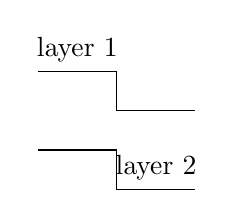
\begin{tikzpicture}
      \draw (0,0) -- (1,0) -- (1,-.5) -- node [above] {layer 2} (2,-.5);
      \draw (0,1) -- node [above] {layer 1} (1,1) -- (1,.5) -- (2,.5);
    \end{tikzpicture}
    \end{minipage}
    \begin{minipage}{.48\linewidth}
      \centering
      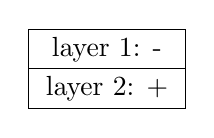
\begin{tikzpicture}
      \draw (0,0) rectangle (2,.5) node [midway] {layer 2: +};
      \draw (0,.5) rectangle (2,1) node [midway] {layer 1: -};
    \end{tikzpicture}
    \end{minipage}
  \end{center}
  Without combinations, they can have a longer lifetime.
  \item Type III: broken gap.
\end{enumext}
% !TeX root = ../main.tex

\chapter{Electrons in a Magnetic Field}

\begin{multline*}
  \text{Free electrons in a magnetic field} \\ \longrightarrow
  \text{Bloch electrons (electrons in a periodic potential field) in a
    magnetic field}
\end{multline*}
For metals, the electrons near the Fermi surface can be considered as the
quasifree electrons, where $m^* \to m$.
So, we start from the free electrons first.

\section{Bohr-Sommerfeld Quantization}

\subsection{Classical Hall effect}

In the polar coordinate
\begin{align*}
  \bm r & = r\cos(\omega t)\bm i + r\sin(\omega t)\bm j\\
  \bm{\dot r} & = -r\omega\sin(\omega t)\bm i + r\omega\cos(\omega t)\bm j\\
  \bm{\ddot r} & = -r\omega^2\cos(\omega t)\bm i - r\omega^2\sin(\omega t)\bm j
\end{align*}
where the equation of motion
\[
  m^*\bm{\ddot r} = e\bm{\dot r}\times\bm B
\]
If the magnetic field $B = (0, 0, B)$, then
\[
  m^*(-r\omega^2\cos(\omega t)) = -e\cdot r\omega\cos(\omega t) B
\]
where $r = v/\omega \propto \frac1B$, and the orbit is quantized.

The current density
\[
  \bm j = \frac{ne^2\tau}{m^*}\bm E
\]
while in Drude model, we have
\[
  \bm j = \hat \sigma \bm E
\]
where $\sigma$ is a tensor mentioned in Chapter 1.
If we apply the magnetic field, we use
\[
  \bm E = \frac{m^*}{ne^2\tau}\bm j + \frac1{ne}\bm j \times \bm B
\]
In the Drude model, the diagonal elements are independent from the magnetic
field, while the $xy$ term is linear to the magnetic field.

\subsection{Bohr-Sommerfeld Quantization rule}

The number of wavelength along the trajectory must be integer
\begin{equation}
  \frac1\hbar \oint \bm p \cdot \d\bm r = 2\pi N
\end{equation}
Apply the magnetic field, we need do the replication $\bm p \to \bm p - e\bm A$,
hence
\begin{equation}
  \frac1\hbar \oint \bm p \cdot \d\bm r - \frac1\hbar \oint e\bm A \cdot \d\bm r
= 2\pi N
\end{equation}
where $\bm p = \hbar\bm k$. Using the motion equation becomes
\begin{equation}
  \hbar\bm k = -e\bm r \times \bm B
\end{equation}
The first term of the integral now becomes
\[
  \frac1\hbar \oint \hbar \bm k \cdot \d\bm r
= -\frac e\hbar \oint(\bm r \times \bm B) \cdot \d r
= -\frac e\hbar \oint \bm B \cdot(\d\bm r \times \bm r) = -\frac{2e}{\hbar} \oint \bm B \cdot \d\bm S = \frac{2e}{\Phi}
\]
and the seconde term
\[
  \frac e\hbar \oint \bm A \cdot \d \bm r \xlongequal{\text{Stock' Equation}}
  \frac e\hbar \oint (\nabla \times \bm B) \cdot \d\bm r
= \frac e\hbar \iint \bm B \cdot \d S = \frac e\hbar \Phi
\]
Hence, the quantization condition becomes
\begin{equation}
  \frac e\hbar \Phi = 2\pi N, \quad \Phi = \frac{2\pi\hbar}{e}N
= \frac he N = \phi_0N
\end{equation}
Since $\phi_0 = BS$, so, the area $S$ should be quantized.
\emph{If the magnetic field is changed, the radius of motion will change
  discretely.}

\subsection{Onsager quantization condition}

Going to $k$-space from $r$-space for $\bm B = (0,0,B_z)$
\[
  \hbar|\bm k| = e|\bm r| B, \quad |\bm k| = \frac{|\bm r|}{l_B^2},
\]
where $l_B = \sqrt{\frac\hbar{eB}}$ denotes the magnetic length.
Then, the area
\[
  S_r = \pi r^2, \quad S_k = \pi k^2, \to S_r = l_B^4 S_k
\]
where $S_k$ denotes the area of \emph{Fermi Surface}. Then, the flux
\[
  \phi = N\phi_0, \quad B l_B^4 S_k = N\frac he
\]
Then, we obtain the the quantization condition in $k$-space
\begin{equation}
  l_B^2 S_k = 2\pi N
\end{equation}
To generalized onsager relation
\[
  l_B^2 S_k = 2\pi\ab(N + \frac12 - \frac\gamma{2\pi})
\]
Consider a change in $B$
\[
  \frac\hbar{eB_N} \cdot S_k = 2\pi N, \quad
  \frac\hbar{eB_{N+1}} \cdot S_k = 2\pi (N + 1)
\]
Hence, the flux area change in $k$-space
\begin{equation}
  S_k \cdot \Delta\ab(\frac1B) = \frac{2\pi}{\hbar} e
\end{equation}

\subsection{Quantization of energy}

Starting from
\begin{gather}
  l_B^2 S_k = 2\pi \ab(N + \frac12 - \frac\gamma{2\pi})\\
  S_k = \pi k^2
\end{gather}
The energy $E = \frac{\hbar^2k^2}{2m}$
\[
  \frac\hbar{eB} \cdot \pi \cdot \frac{2mE}{\hbar^2} = 2\pi(N + \frac12), \quad
  E = \hbar\omega\ab(N + \frac12)
\]

\subsection{Full quantum mechanical solution}

The Hamiltonian for a free electron
\[
  \hat H = \frac{\hat p^2}{2m} \xlongrightarrow{\bm p\to\bm p - e\bm A}
  \frac{(\bm p - e\bm A)^2}{2m}
\]
where $\bm B = \nabla \times \bm A$ and use Landau gauge $\bm A = (0,Bx,0)$.
Since $p_y$, $p_z$ commutes with the Hamiltonian, it can be replaced with its
eigenvalue $\hbar k_y$, $\hbar k_z$. The Schr\"odinger equation becomes
\[
  \ab[\frac{p_x^2}{2m^*}
    + \frac1{2m^*}(\hbar k_y - eB_x)^2 + \frac{\hbar^2k^2}{2m^*}]\psi
= E\psi
\]
Rearrange it
\[
  \ab[\frac{p_x^2}{2m^*}
    + \frac1{2m^*}(\hbar k_y - eB_x)^2]\psi
= \ab(E - \frac{\hbar^2k^2}{2m^*})\psi = E'\psi
\]
Denote $x_0 = \frac{\hbar k_y}{eB}$, the Schr\"odinger equation becomes
\begin{equation}
  \ab[\frac{p_x^2}{2m^*}
    + \frac12m^*\omega_c^2(x - x_0)^2]\psi = E'\psi
\end{equation}
The quantized energy
\begin{equation}
  E = \frac{\hbar^2k_z^2}{2m^*} + \ab(N + \frac12)\hbar\omega_c
\end{equation}

Due to the limitation of boundary,
\[
  0 < x_0 = \frac{\hbar k_y}{eB} < L_x
\]
where $k_y = \frac{2\pi}{L_y}n_y$, $\Delta k_y = \frac{2\pi}{L_y}$, it will be
limited within
\[
  0 < k_y < \frac{eBL_x}{\hbar`'}
\]
So, the total number of state
\[
  n = \frac{eBL_x/\hbar}{2\pi/L_y} = \frac{eB(L_xL_y)}{h}
\]
and the density of states
\[
  \text{DOS} = \frac{eB(L_xL_y)/\hbar}{L_xL_y}g_s = \frac{eB}{h}g_s
= \phi_0 B g_s \propto B
\]
Usually, $g_s = 2$, but for like graphene, $g_s > 2$.
By increasing the magnetic field, one can confine all of the electrons within
the same energy (such as the ground) state.

\section{Landau Quantization}

\subsection{Filling factor}

With a given $E_f$, the number of Landau levels filled with states $\nu$.
\begin{equation}
  \nu = \frac{n}{eB/h} = \frac{hn_B}{eB}
\end{equation}
The Landau level will broaden due to scattering.
For a given scattering time $\tau_q$, the broaden energy
\[
  \Delta E \sim \frac\hbar{\tau_q}
\]
due to Heisenberg's uncertainty principle.
When $\Delta E > \hbar\omega_c$, or $\frac\hbar{\tau_c} > \hbar\omega_c$,
$\omega_c\tau_c < 1$. We denotte $\mu = e\tau/m$, then
\[
  \omega_c \cdot \frac{\mu m^*}{e} = \frac{eB}{m^*} \frac{\mu m^*}{e} < 1,
  \quad B \mu_q < 1
\]
So, when $B\mu_q \geq 1$, we could not distinguish the levels.
where $\mu_q$ denotes the quantum mobility. E.g, for
$B = \qty 1\T$, $\mu_q \to \qty{e3}{\cm/\N\cdot\s}$.

\section{Shubnikov-de Hass Oscillators}

\subsection{Zeeman splitting}

Each Landau level will separate into two levels.
\[
  E_c = \hbar \frac{eB}{m^*}, \quad E_z = g\mu_B B
\]
In case that $E_c < E_z$, then $\hbar eB/m^* < g\mu_B B$,
$\hbar eB < gm^*\mu_B B$.

If tune $B$ to $B_z$ and $B_\parallel$, then
\[
  \frac{E_c}{E_B} = \frac{\frac{\hbar eB}{m^*}\cos\theta}{g\mu_B B}
= \frac{\hbar e\cos\theta}{gm^*\mu_B}
\]

\section{Integer Quantum Hall Effect}

\subsection{Edge modes}

The Hamiltonian with the potention $\phi(x)$
\begin{equation}
  \hat H = \frac{p_x^2}{2m^*} + \frac1{2m^*}(\hbar k_y - eBx)^2 + \phi(x)
\end{equation}
The eigenenergy will be
\[
  E(\hbar k) = \ab(N + \frac12)\hbar\omega_c + \phi\ab(\frac{\hbar k_y}{eB})
\]
The current
\[
  I = -e \int_{-\infty}^\infty \frac{\d k}{2\pi} v_y(k)
= \frac{e}{2\pi l_B^2} \int_0^x \d x \frac1{eB} \fdv\phi x
= \frac e{2\pi\hbar} \Delta\mu
\]
where $\pdv E{k_y} = \pdv\phi x \cdot \ab(\frac\hbar{eB})$.
In the bulk, the electrons motion counterclockwise; But on the both edges
of top and top, the electrons will be ``perfectly scattered'' (reflected) by the
edges and do hafl-circle counterclockwise motion.
Obviously, the direction of the currents is different.

\section{Fractional Quantum Hall Effect}

\subsection{Composite fermions}

\[
  B = n_e\phi_e (2j + 1/\nu^*)
\]
Then, $\nu = \frac{\nu^*}{2j\nu^* + 1}$.

If consider $j = 1$, which means that each electrons attached to flux, then
\[
  \nu = \frac13, \rightarrow \nu^* = 1.
\]

\subsection{Wigner crystal}

The electron-electron interaction is so large that forms the lattice.
The bonds are Columb interactions.
When a strong filed is applied on a level, the electrons will be fixed and form
the lattice.
% !TeX root = ../main.tex

\chapter{Dirac Band Theory}

\section{Introduction to Graphene}

\paragraph{Why $\mu$ in graphene is very high}
\begin{enumext}
  \item Dirac band: $m^* = 0$.
  \item Electron-phonon scattering is weak.
  \item $\tau_i$ increase: $\mu_i$ increase.
\end{enumext}

\subsection{Honeycomb lattice and its Brillouin zone}

Two vectors
\[
  a_1 = \frac a2(1,\sqrt3), \quad
  a_2 = \frac a2(1,-\sqrt3)
\]
\begin{paracol}{2}
We want to get the $E(k)$ relation, so we obtain the reciprocal lattice first
\[
  b_1 = \frac{2\pi}{a}\ab(1, \frac{\sqrt3}{3}),\quad
  b_2 = \frac{2\pi}{a}\ab(-1, \frac{\sqrt3}{3}).
\]
with the first Brillouin zone
\[
  k = \frac{4\pi}{3a}(1,0), \quad k' = \frac{4\pi}{3a}(-1,0).
\]
\switchcolumn \centering
  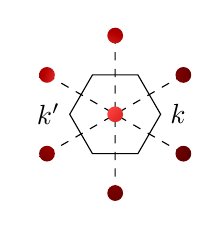
\begin{tikzpicture}
    \draw
      (0:{1/sqrt(3)}) node [right] {$k$} --  (60:{1/sqrt(3)}) --
      (120:{1/sqrt(3)}) -- (180:{1/sqrt(3)}) node [left] {$k'$} --
      (240:{1/sqrt(3)}) -- (300:{1/sqrt(3)}) -- cycle;
    \draw [dashed]
      (150:1) -- (150:-1)
      (90:1) -- (90:-1)
      (30:1) -- (30:-1);
    \shade [ball color = red]
      (0,0) circle (.1)
      (30:1) circle (.1)
      (90:1) circle (.1)
      (150:1) circle (.1)
      (210:1) circle (.1)
      (270:1) circle (.1)
      (330:1) circle (.1);
  \end{tikzpicture}
\end{paracol}

\subsection{Tight-binding method to calculate band structure of graphene}

The Boloch wave function
\begin{align}
  \psi_A & = \frac1{\sqrt N} \sum_{\bm R_A}^N \upe^{\iu\bm k \cdot \bm R_A}
    \varphi_A(\bm r - \bm R_A),\\
  \psi_B & = \frac1{\sqrt N} \sum_{\bm R_B}^N \upe^{\iu\bm k \cdot \bm R_A}
    \varphi_B(\bm r - \bm R_B)
\end{align}
where $\psi_A$ denotes the atomic orbital of A-atom, also for $\psi_B$.
The total wavefunction
\begin{equation}
  \psi = \sum_n b_n\psi_n = b_A \psi_A + b_B \psi_b
= b_A \frac1{\sqrt N} \sum_{R_A} \upe^{\iu\bm k \cdot\bm R_A}
  \varphi_A(\bm r - \bm R_A) +
  b_B \frac1{\sqrt N} \sum_{R_B} \upe^{\iu\bm k \cdot\bm R_B}
  \varphi_B(\bm r - \bm R_B)
\end{equation}
The eigen function
\[
  \hat H\ket|\psi> = E\ket|\psi>
\]
Project all the wavefunction of A-atom
\[
  \braket<\psi_A|\hat H|\psi> = E\braket<\psi_A|\psi>
\]
Then, we have
\begin{multline}
  b_A \frac1{\sqrt N} \sum_{R_A} \upe^{\iu\bm k \cdot\bm R_A}
  \braket<\varphi_A|\hat H|\varphi_{A'}(\bm r - \bm R_A)> +
  b_B \frac1{\sqrt N} \sum_{R_B} \upe^{\iu\bm k \cdot \bm R_B}
  \braket<\varphi_A|\hat H|\varphi_B(\bm r - \bm R_B)>\\
= E\ab[b_A\frac1{\sqrt N} \sum_{R_A}\upe^{\iu\bm k\cdot \bm R_A}
    \braket<\varphi_A|\varphi_A(\bm r - \bm R_A)> +
    b_B \frac1{\sqrt N} \sum_{R_A} \upe^{\iu\bm k\cdot\bm R_B}
    \braket<\varphi_A|\varphi_B(\bm r - \bm R_B)>]
\end{multline}
Rearrange it
\[
  b_A\braket<\varphi_A|\hat H|\varphi_B> \upe^{\iu\bm k\cdot \bm R_A}
+ b_B\braket<\varphi_A|\hat H||\varphi_B> \sum_{R_B}\upe^{\iu\bm k\cdot \bm R_B}
= E b_A \upe^{\iu\bm k\cdot\bm R_A}
\]
Substitute the orthonormality
$\braket<\varphi_A|\varphi_B> = \delta_{A,B}\epsilon_{A,B}$
\[
  b_A\epsilon_0 + b_Bt\sum_{i = 1,2,3} \upe^{\iu k\cdot k_i} = Eb_A
\]
Finally, we arrive at
\begin{equation}
  b_A\epsilon_0 + b_Bt\sum_i \upe^{\iu k\cdot \delta_i} = E b_a,
\end{equation}
Similarly, we can project by $\bra<\varphi_B|$
\begin{equation}
  b_At\sum_i \upe^{-\iu \bm k\cdot \bm \delta_i} + b_B\epsilon = E b_B
\end{equation}
we define
\[
  f(k) = \sum_i \upe^{\iu\bm k \cdot \bm \delta_i}
\]
Then, we can write them into matrix,
\begin{equation}
  \begin{pmatrix}
    \epsilon_0 & tf(k)\\
    tf^*(k) & \epsilon
  \end{pmatrix}
  \begin{pmatrix}
    b_A\\b_B
  \end{pmatrix} = E
  \begin{pmatrix}
    b_A\\b_B
  \end{pmatrix}, \mathbf A\bm b = E\bm b
\end{equation}
The determine $\det(\mathbf A - \lambda\identity)$ should be zero
\[
  \begin{vmatrix}
    \epsilon_0 - E & tf(k)\\
    tf^*(k) & \epsilon_0 - E
  \end{vmatrix} = 0
\]
We can obtain the $E(k)$ relation
\begin{equation}
  E = \epsilon_0 \pm t|f(k)|.
\end{equation}
Make the replacement
\[
  \bm K = \frac{4\pi}{3a}(1,0) \to (0,0), \quad \bm q = \bm k - \bm K, \quad
  \bm p = \hbar\bm q
\]
Then
\begin{align}
  f(k) & = \upe^{\iu\bm k_xa/\sqrt3}
       + 2\upe^{\iu-\iu k_xa/2\sqrt3}\cos(k_xa/2)
= \upe^{\iu q_ya/\sqrt3} + 2\upe^{\iu q_ya/2\sqrt3},\\
  f(q) & = \cos\ab[\frac{(q_x + \frac{4\pi}{3a})a}{2}]
= \upe^{\iu q_ya/\sqrt3} + 2\upe^{-\iu q_ya/2\sqrt3}
  \ab(\cos\frac{q_xa}{2} \cos\frac{4\pi}{3} - \sin\frac{q_xa}{2} \sin\frac{4\pi}{3})
\end{align}
Expand $f(q)$ to the first order
\begin{equation}
  f(q) = \frac{\sqrt3a}{2} (\iu q_y - q_x) + \iu \frac{a^x}{4} q_x \cdot q_y
= \frac{\sqrt3a}{2}(\iu q_y - q_x)
\end{equation}
We can rewrite
\[
  E(k) = \pm t|f(k)| = \pm t\frac{\sqrt3a}{2\hbar} |q|\hbar = v_F |\bm p|
\]
One can rewrite the Hamiltonian interms of Pauli matrices
\begin{equation}
  H_k(p) = v_F(\sigma_x p_x + \sigma_y p_y) = v_F \bm \sigma \cdot \bm p
\end{equation}

\section{Calculation about TBC}

Using the approximation
\begin{enumext}
  \item Only consider the nearest neighbor hopping
  \[
    \braket<\phi_A|H|\phi_B> \neq 0
  \]
  \[
    \epsilon_0 = 0, \quad E_\pm = \pm V_0|f(\bm k)|
  \]
  \item $f(\bm k) \approx \frac{\sqrt3}{2} a(\iu q_y - \xi q_x)$.
\end{enumext}

\section{Chirality}

\begin{enumext}
  \item For conduction band electron: $\bm\sigma \cdot \bm n = 1$.
  \item For valence band electron: $\bm\sigma \cdot \bm n = -1$.
\end{enumext}

\section{Dirac equation with a mass}

The Hamiltonian
\[
  H_k =
  \begin{pmatrix}
    \Delta & -\gamma_0f(\bm k)\\
    -\gamma_0f^*(\bm k) & -\Delta
  \end{pmatrix}
\]
The energy
\[
  E_\pm = \pm\sqrt{\Delta^2 + (\gamma_0|f(\bm k)|)^2}
= \pm \sqrt{(m_Dv_F^2)^2 + (\hbar v_Fk)^2}
\]
where $m_D = \Delta/v_F^2$.
The gap is
\[
  \Delta E = E_+ - E_-
= 2\sqrt{\Delta^2 + (\gamma_0|f(\bm k)|)^2},
\]
and we can open a gap in the band.

\section{Density of states in Graphene}

\[
  g(E) = g_sg_vvv \frac{|E|}{2\pi\hbar^2v_F^2}
\]
The total carrier density
\[
  n = \int_0^\infty g(E) f(E) \d E
= \int_0^{E_f} \frac{g_sg_N E}{2\pi\hbar^2v_F^2} \d E
= \frac{g_sg_VE}{2\pi\hbar^2v_F^2}\d E
= \frac{g_sg_V}{2\pi\hbar^2v_F^2} \frac12 E_F^2
= \frac{E_f^2}{\pi\hbar^2v_F^2}
\]
where $E_F = \pm\hbar v_F\sqrt{|n|\pi} = \pm\hbar v_Fk_F$.

\section{Massless Dirac fermions}

\[
  m^* = \frac1\hbar/\pdv[2]Ek
\]
For $E = \hbar v_F k$, $\pdv Ek = \hbar v_F$, and $\pdv[2]Ek = 0$,
the effective mass will diverge.
So, for massless particle, $m_0 = 0$, $E = c|p|$.

\section{Bilayer Graphene}

The matrix formations of Schr\"odinger equation
\begin{equation}
  \begin{pmatrix}
    H_{AA} & H_{AB}\\
    H_{BA} & H_{BB}
  \end{pmatrix}\psi =
  \begin{pmatrix}
    \braket<\phi_A|\phi_A> & \braket<\phi_A|\phi_B>\\
    \braket<\phi_B|\phi_A> & \braket<\phi_B|\phi_B>\\
  \end{pmatrix}\psi
\end{equation}
For the nearest hopping, the vectors are defined: $\bm\delta_1$, $\bm\delta_2$,
$\bm \delta_3$ with $\braket<\phi_A|H|\phi_B> \neq 0$.
\begin{paracol}{2}
There are two ways for stacking: $A-A$ stacking and $A-B$ stacking.
The former one is unstable, so we consider the latter one only.

Denote the hopping parameter between $A_i$ and $B_i$ is $\gamma_0$, so
\[
  \gamma_0 = \braket<\phi_{A_1}|H|\phi_{B_1}>
= \braket<\phi_{A_2}|H|\phi_{B_2}>
\]
\switchcolumn \centering
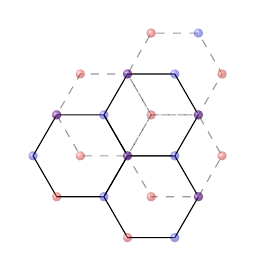
\begin{tikzpicture}[scale = .6]
  \foreach \i in {0,120,240}
    \draw [rotate around = {\i:(0,0)}]
          (0,0) --++ (0:1) --++ (-60:1) --++ (-120:1) --++
          (-180:1) --++ (-240:1) --++ (60:1);
  \begin{scope}[opacity = .4]
  \foreach \i in {0,120,240}
    {
      \shade [rotate around = {\i:(0,0)}, ball color = red]
        (0,{sqrt(3)}) circle (.1);
      \shade [rotate around = {\i:(0,0)}, ball color = red]
        (1.5,{sqrt(3)/2}) circle (.1);
      \shade [rotate around = {\i:(0,0)}, ball color = blue]
        (1,0) circle (.1);
      \shade [rotate around = {\i:(0,0)}, ball color = blue]
        (1,{-sqrt(3)}) circle (.1);
    }
  \shade [ball color = red] (0,0) circle (.1);
  \end{scope}
  \begin{scope}[opacity = .4, shift = {(60:1)}]
  \foreach \i in {0,120,240}
    \draw [dashed, rotate around = {\i:(0,0)}]
          (0,0) --++ (0:1) --++ (-60:1) --++ (-120:1) --++
          (-180:1) --++ (-240:1) --++ (60:1);
  \foreach \i in {0,120,240}
    {
      \shade [rotate around = {\i:(0,0)}, ball color = red]
        (0,{sqrt(3)}) circle (.1);
      \shade [rotate around = {\i:(0,0)}, ball color = red]
        (1.5,{sqrt(3)/2}) circle (.1);
      \shade [rotate around = {\i:(0,0)}, ball color = blue]
        (1,0) circle (.1);
      \shade [rotate around = {\i:(0,0)}, ball color = blue]
        (1,{-sqrt(3)}) circle (.1);
    }
  \shade [ball color = red] (0,0) circle (.1);
  \end{scope}
\end{tikzpicture}\hfill
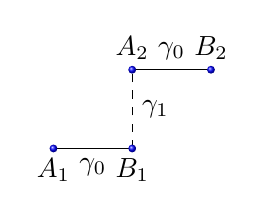
\begin{tikzpicture}
  \draw (-1,0) -- node [below] {$\gamma_0$} (0,0) (0,1) --
   node [above] {$\gamma_0$} (1,1);
  \draw [dashed] (0,0) -- node [right] {$\gamma_1$} (0,1);
  \shade [ball color = blue] (-1,0) circle (.05) node [below] {$A_1$};
  \shade [ball color = blue] (0,0) circle (.05) node [below] {$B_1$};
  \shade [ball color = blue] (0,1) circle (.05) node [above] {$A_2$};
  \shade [ball color = blue] (1,1) circle (.05) node [above] {$B_2$};
\end{tikzpicture}
\end{paracol}
also consider the hopping between $A_i$ and $B_j$, another nearest hopping
the hopping between $A_i$ and $A_j$ can be ignored.
We can write the Sch\"odinger with a labeled Hamiltonian matrix,
the crossing elemets correspoondings to the hopping between the labels.
\[
  \begin{pNiceMatrix}[first-row, last-col]
    A_1 & B_1 & A_2 & B_2\\
    \epsilon_0 - E & -\gamma_0 f(k) & 0 & 0 & A_1\\
    -\gamma_0 f^*(k) & \epsilon_0 - E & \gamma_1 & 0 & B_1\\
    0 & \gamma_1 & \epsilon_0 - E & -\gamma_0 f(k) & A_2\\
    0 & 0 & -\gamma_0 f^*(k) & \epsilon_0 - E & B_1
  \end{pNiceMatrix}\, \bm\psi = 0
\]
where $\epsilon_0$ is a constant value: the site energy;
and $f(k) = \sum_{i=1}^3 \upe^{-\iu k \cdot \delta_k}$.
We can obtain two energies
\begin{equation}
  E_\pm^\alpha = \pm\frac{\gamma_1}{2} \ab(
    \sqrt{1 + \frac{4\gamma_0^2|f(k)|^2}{\gamma_1^2}} + \alpha)
\end{equation}
where $\alpha = \pm 1$.
\begin{enumext}
  \item $\alpha = +1$: $k$, $k'$ valley, $f(k) = 0$,
  \begin{equation}
    E_\pm^{+1} = \pm \frac{\gamma_1}{2} \times 2 = \pm \gamma_1
  \end{equation}
  \item $\alpha = -1$: $f(k) = 0$
  \begin{equation}
    E_\pm^{-1} = \pm\frac{\gamma_1}{2} (1 - 1) = 0,
  \end{equation}
  and the two bands will touch each other.
\end{enumext}
Around K point, $f(\bm k) \to 0$, so $|\gamma_0 f(\bm k)| \ll |\gamma_1|$.
Denoting $m^* = \frac{\gamma_1}{2v_F^2}$, so, the $2\times2$ Hamiltonian can be
expressed by
\begin{equation}
  H_2 =
  \begin{pmatrix}
    0 & -\frac{\gamma_0^2 f^2(\bm k)}{\gamma_1}\\
    -\frac{\gamma_0^2(f^*(\bm k))}{\gamma_1} & 0
  \end{pmatrix} = -\frac1{2m^*}
  \begin{pmatrix}
    0 & (\xi p_x - \iu p_y)^2\\
    (\xi p_x + \iu p_y)^2 & 0
  \end{pmatrix}
= -\frac{p^2}{2m^2} \bm \sigma \cdot \bm n_2
\end{equation}
One can also call $m^*$ the massive Dirac fermions.

\paragraph{Extension}

For $N$-layer graphene: $E(k) \sim k^N$.
The energy bands get flatter as $N$ increasing, which will get a larger density
of states.

\subsection{Bilayer graphere under an electric field}

By applying an electric field parallels to $z$-axis,
the on-site energies will be different
\[
  \braket<\phi_{A_1}|H|\phi_{A_1}> \neq
  \braket<\phi_{A_2}|H|\phi_{A_2}>
\]
There will a band gap $\Delta$.

\section{Landau Levels in Graphene}

Previous, we've discussed the free electron, so, the Landau
quantization
\[
  E = \hbar\omega\ab(N + \frac12)
\]
which is based on the parabolic relation $\frac{p^2}{2m}$.

In mono graphene, since the Hamiltonian
\[
  H = v_F \bm\sigma \cdot \bm p
\]
we will get a different dispersion relation.
Starting from
\begin{equation}
  H = v_F \bm \sigma \cdot \bm p = v_F
  \begin{pmatrix}
    0 & p_x - \iu p_y\\
    p_x + \iu p_y & 0
  \end{pmatrix}
\end{equation}
Replace $\bm p \to \bm - \bm A$,
then using Landau gauge: $A_x = 0$, $A_y = Bx$, $A_z = 0$
\[
  q_x \to z_x,\ q_y \to q_y - x/l_B^2,\ l_B = \sqrt{\hbar/eB}
\]
The Hamiltonian becomes
\[
  H = \hbar v_F
  \begin{pmatrix}
    0 & q_x - \iu\ab(q_y - \frac x{l_B^2})\\
    q_x + \iu\ab(q_y - \frac x{l_B^2}) & 0
  \end{pmatrix}
\]
Define the operator $a = \frac1{\sqrt2l_B}(\tilde x + \iu l_B^2 q_x)$, we have
$[a,a^\dagger] = 1$. The Hamiltonian
\[
  H = \hbar v_F
  \begin{pmatrix}
    0 & q_x + \frac{\iu\tilde x}{l_B^2}\\
    q_x - \frac{\iu\tilde x}{l_B^2} & 0
  \end{pmatrix} = \frac{\sqrt2\hbar v_F}{l_B}
  \begin{pmatrix}
    0 & \iu a^\dagger\\
    -\iu a & 0
  \end{pmatrix}
\]
from 1D quantm harmonic oscillator, we \emph{guess} the eigenstates to be
\[
  \ket|\psi_n> =
  \begin{pmatrix}
    A_n\ket|n> \\ B_n\ket|n - 1>
  \end{pmatrix}
\]
Apply $H$ to it, one can obtain
\begin{gather*}
  B_n \sqrt2\hbar v_F \iu \sqrt n = E A_n,\\
  A_n \frac{\sqrt2\hbar v_F}{l_B} (-\iu \sqrt n) = EB_n.
\end{gather*}
Multiply them, we can obtain the energy
\[
  E_n = \pm v_F \sqrt{2\hbar eB|n|}
\]
which is promotional to $\sqrt B$.

\appendix
\sidefoot \thepage
\fancyhead[OL, ER]{Mingyu Xia (Westlake ID: 20251202247)}
\fancyhead[EL]{\sffamily \rightmark}
\fancyhead[OR]{\fontfamily{lmr}\selectfont<<\texttt{%
  \href{mailto:xiamingyu@westlake.edu.cn}{xiamingyu@westlake.edu.cn}}>>}
\addcontentsline{toc}{chapter}{Problem Set}
\renewcommand *\familydefault {\sfdefault}

\renewcommand *\newweek {\refstepcounter{week}}
\pagestyle{empty}
\pgfpagesuselayout{resize to}[a4paper]
\newgeometry{hmargin = .2in, vmargin = -.2in}
\pgfpagesuselayout{8 on 1}[a4paper, landscape]
\setlength \abovedisplayskip {3.6pt}
\setlength \belowdisplayskip {3.6pt}
\linespread{1.12}
\begin{multicols}{2}
% % !TeX root = ../main.tex

\begin{framed}\large\bfseries
  \#2 Free Electron Model of Metals
\end{framed}

\paragraph{Drude model}\leavevmode

\subparagraph{Basic assumptions}\leavevmode

\begin{enumext*}[nosep, columns = 5, label = (\alph*)]
  \item(5) Free electron approximation
  \item(5) Electrical resistance results from scattering
  (all information is lost upon scattering).
  \item(3) Relaxation-time approximation.
  \item(2) Thermal equilibrium.
\end{enumext*}

\subparagraph{With(out) electric field}

Free electron moving randomly, no net current;
Or the drift velocity $v_d \ll v_\text{rms}$.

\subparagraph{EOM}

\begin{enumext}[nosep]
  \item Let $\tau$ be the scattering time and $1/\tau$ be the scattering rate.
  \item In $\d t$, a fraction $\frac{\d t}\tau$ of the electrons are scattered
  with zero average velocity.
  \item The rest part $1 - \d t/\tau$ are accelerated by external force $-eE$.
  \item In $t \sim t + \d t$, the EOM (omit high-order terms)
  \[
    m\odv{\bm v}/t = -m\bm v/\tau - e\bm E
  \]
  At steady state ($\odv{\bm v}t = 0$). The drift velocity
  \[
    \bm v_d \equiv \braket<\bm v(t)> = -e\tau\bm E/m \equiv -\mu\bm E,
  \]
  where mobility $\mu = \frac{\bm v}{\bm E} = \frac{e\tau}{m}$.
  For a given field, a higher $\mu$ means the electrons will move faster.
  The conductance
  \[
    \sigma = \bm j/\bm E
  = -en\bm v/\bm E = ne\mu = -e^2n\tau/m^*.
  \]
  Here, $\tau = l/v_\text{rms}$ is usually independent of $E$.
\end{enumext}

\subparagraph{Classical Hall effect}

\begin{enumext}
  \item Classically, electrons experience
  $\bm F = -e(\bm E + \bm v \times \bm B)$
  \item Cyclotron motion: $\bm E = 0$
  \[
    \ddot x + \ab(eB_z/m^*)^2x = 0, \enspace
    \omega_c = eB/m^*, \enspace
    r_c = v/\omega_c \propto 1/B.
  \]
  Classically, any orbit size is allowed.
\end{enumext}

\subparagraph{Drude model with a magnetic field}\leavevmode

Consider Drude model with applied electric and magnetic fields
\[
  m^*\dot{\bm v} = -e(\bm E + \bm v \times \bm B) - m^*\bm v/\tau
\]
Taking the steady state, with Ohm's rule $\bm j = -ne\bm v = \hat\sigma \bm E$
\begin{gather*}
  \hat\sigma =
  \begin{pmatrix}
    \frac{\sigma_0}{1 + \omega_c^2\tau^2} &
    \frac{\sigma_0\omega_c\tau}{1 + \omega_c^2\tau^2} & 0\\
   -\frac{\sigma_0\omega_c\tau}{1 + \omega_c^2\tau^2} &
    \frac{\sigma_0}{1 + \omega_c^2\tau^2} & 0\\
    0 & 0 & \sigma_0
  \end{pmatrix},\
  \hat\rho = \hat\sigma^{-1},\
  \sigma_0 = \frac{ne^2\tau}{m^*}.
\end{gather*}
The Hall coefficient $R_H = \rho_{xy}/B = -1/ne$.

\subparagraph{Drawbacks}

\begin{enumext*}[label = (\alph*), nosep, columns = 7]
  \item(3) Existence of insulators.
  \item(4) Temperature dependence of $\sigma$.
  \item(7) Heat capacity $C_v^\text D = \frac32nk_B$ does not match
  $C_v \approx 10^{-4} nk_BT$.
\end{enumext*}

\paragraph{Summerfeld model for electrons in metals}

\begin{enumext}
  \item Electrons treated quantum mechanically:
  Quantize the energy of electron gas.
  \item The electronic velocity distribution is given by the quantum
  Fermi-Dirac distribution.
  \item Pauli exclusion: At most one electron can occupy any single
  electron level.
\end{enumext}

\subparagraph{Electron wave}\leavevmode

Schr\"odinger equation for free electron
$\nabla^2\psi(\bm r) = -\frac{2mE}{\hbar^2}\psi(\bm r)$.
The solution is a plane wave with the energy
\[
  \psi(\bm r) = \frac1{\sqrt V} \upe^{\iu(k_xx + k_yy + k_zz)},\enspace
  E = \frac{\hbar^2(k_x^2 + k_y^2 + k_z^2)}{2m}.
\]

\subparagraph{Born-von Karman periodic boundary conditions}\leavevmode

The electrons are confined in a 3D box ($V = L_xL_yL_z$) with
\begin{enumext}[columns = 2]
  \item $U(\bm r) = 0$ inside the box,
  \item $U(\bm r) = \infty$ outside the box.
\end{enumext}
The PBC can be applied
\[
  \psi(x + L_x, y, z) = \psi(x, y + L_y, z) = \psi(x, y, z + L_z)
= \psi(x, y, z),
\]
determines the allowed $k$
\[
  \upe^{\iu k_iL_i} = 1,\quad k_i = 2\pi n_i/L_i, \quad n_i \in \mathbb Z.
\]
The boundary conditions lead to quantization.

\subparagraph{States in $k$-space}\leavevmode

\begin{enumext}
  \item The allowed quantum states can be visualized as a 3D grid of points in
  $k$-space with the distance of $\Delta k_i = 2\pi/L_i$.
  \item In $k$-space, one grid point occupies
  $\prod_{x,y,z}(\frac{2\pi}{L_i}) = (2\pi)^3/V$.
  \item There are $2 \times V/(2\pi)^3$ (Each grid point can be occupied
  by $\ket|\uparrow>$, $\ket|\downarrow>$) quantum states per unit
  volume in k-space.
\end{enumext}

\subparagraph{Fermi energy}\leavevmode

\begin{enumext}
  \item The free electron gas is isotropic, so the surface of constant
  $E = \hbar^2(k_x^2 + k_y^2 + k_z^2)/2m$ in k-space is a sphere.
  \item Fermi energy: energy of the highest occupied state at zero temperature.
  \begin{enumext}
    \item Number of
    electrons: $N = 2 \times \frac{4\pi k_F^3/3}{(2\pi/L)^3} = k_F^3V/3\pi^2$.
    \item Fermi wave vector: $k_F = (3\pi^2n)^{1/3}$, $n = N/V$ denotes the
    carrier density.
    \item Fermi
    energy: $E_f = \hbar^2k_F^2/2m = \frac{\hbar^2}{2m}(3\pi^2n)^{2/3}$.
    \item Fermi velocity and temperature relate to the Fermi
    energy $E_F = \frac12mv_F^2 = k_BT_F$.
  \end{enumext}
\end{enumext}

\subparagraph{Bosons and Fermions at $T = 0$}

\begin{enumext}
  \item Bosons: The occupation number can take on any value:
  photons, mesons, any composite particles with integer spin.
  \item Fermions: The occupation number can be zero or one due to the Pauli
  exclusion principle: lectrons, protons, neutrons, any composite
  particles with half-integer spin.
\end{enumext}

\subparagraph{Bosons and Fermions at $T \neq 0$}\leavevmode

At finite temperature, Bosons/Fermions obeys Bose-Einstein/Fermi-Dirac
statistics $\bar n_i = g_i\{\exp[(\epsilon_i-\mu)/k_BT] \mp 1\}^{-1}$.
\begin{enumext}[columns = 2]
  \item $\epsilon_i$: Energy of the $i$-th state.
  \item $n_i$: Occupation number.
  \item $g_i$: Degeneracy.
  \item $\mu$: Chemical potential.
\end{enumext}
Bosons and Fermions are identical and indistinguishable particles

\subparagraph{The electron gas at zero temperature}

\begin{enumext}
  \item  All quantum sates inside the Fermi sphere are filled while outside
  are empty.
  \item The surface of the Fermi sphere is called Fermi surface.
\end{enumext}

\subparagraph{Fermi-Dirac distribution}\leavevmode

Probability distribution function $f(E)$: the probability that a state
with energy $E$ is occupied.
\[
  f(E) = [1 + \upe^{(E-E_f)/k_BT}]^{-1} \xlongrightarrow{T=0}
  \begin{cases}
    0, & E > E_f,\\
    1, & E \leq E_f.
  \end{cases}
\]
As $T$ increasing, the function will broaden $\sim 2k_BT$ at $E = E_f$.
\begin{enumext}
  \item At Fermi level, the probability being occupied is always $1/2$.
  \item $E_f(T = 0) = E_F$, $E_f(T > 0) < E_F$
\end{enumext}

\subparagraph{Density of states}

The number states can be occupied per energy.
\[
  g(E) = \odv nE = \frac1V\odv NE =
  \begin{cases*}
    \frac{m^*}{\pi^2\hbar^3}\sqrt{2m^*E}, & 3D,\\
    \frac1{\pi\hbar} \sqrt{2m^*/E},       & 1D,\\
  \end{cases*}\
  \begin{array}{ll}
    m^*/\pi\hbar^2,                       & 2D,\\
    2\delta(E),                           & 0D.
  \end{array}
\]

\subparagraph{The electron gas at $T > 0$}

\begin{enumext}
  \item The total number of electron at $T > 0$
  \[
    n = N/V = \int_0^\infty g(E) [\upe^{(E-E_f)/k_BT} + 1]^{-1} \d E.
  \]
  \item  The energy
  density $u = U/V = \int_0^\infty Eg(E) \frac1{\upe^{(E-E_f)/k_BT} + 1} \d E$.
\end{enumext}

\subparagraph{Current density}

\[
  \bm j =-ne\bm v = -2e \int \frac{\d^3\bm k}{(2\pi)^3} f(\bm k) v(\bm k).
\]
At zero field, for every occupied state $\bm k$, there is a state $-\bm k$
occupied with the same probability. Therefore, $\bm j = 0$.

In Drude model, assume that scattering adds damping
\[
  \odv{\hbar\bm k(t)}t = -e\bm E - \frac{\hbar[\bm k(t) - \bm k]}{\tau}
  \xlongrightarrow[\text{steady state}]{t=\infty} \bm k(t)
= \bm k - \frac{e\tau}{\hbar}\bm E,
\]
the wave vector of every electron is shifted. The current density
\[
  \bm j = -2e\int \frac{\d^3\bm k}{(2\pi)^3}
          f\ab(\bm k + \frac{e\tau}\hbar\bm E) v(\bm k)
        \xlongequal{\int\d^3\bm k f(\bm k)\bm k = 0}
        \frac{e^2\tau}{m}n\bm E
\]
with $\bm j = \sigma\bm E$, $\sigma = ne^2\tau/m$ the same as that in
Drude model.

The excess current carriers are only those very near the Fermi surface.
So the current carriers have velocity $v_F$.

\subparagraph{Heat capacity of an electron gas}

At low temperature, $\mu \sim E_f$ and $\pdv{f(E,T)}T$ is peaked close to $E_f$,
$k_BT \ll E_f$. Then
\[
  C_e = \pdv{\Delta U}/T \approx \pi^2 nk_B^2T/2T_f \propto T.
\]
The heat capacity of electrons increases linearly with temperature.

\subparagraph{Limitation of Free electron gas model}

\begin{enumext}
  \item Cannot explain semiconductors/insulators.
  \item $C_V \propto T$ only at very low $T$.
  \item Fail to explain $C_V \sim T^3$ at intermediate temperature region.
  \item Wiedemann-Franz law temperature dependent.
  \item The sign of Hall coefficient $R_H = -1/ne$.
\end{enumext}

\begin{framed}\large\bfseries
  \#3 Lattice Vibrations and Phonons
\end{framed}

\subparagraph{Specific heat capacity in solids}

Experimentally, $C_V \sim aT + bT^3$ (electronic and lattice).
At high $T$, $C_V$ approaches constant.

\subparagraph{Dulong-Petit law}

Each atom has $3$ independent harmonic oscillators; each contributes $k_BT$ to
energy. Thus, $C_V = 3N_Ak_B = 3R$.
\begin{enumext}
  \item Only applicable to heavier elements (fail for light and
  strongly bonded atoms, such as diamond)
  \item Appliable only at high temperatures.
\end{enumext}

\paragraph{Einstein model}

Assume \emph{independent harmonic oscillators} with Einstein
frenquency $\omega_E$ and quantized
energy $E_n = \hbar\omega_E\ab(n + \frac12)$.

$N$ vibrating atoms need $3N$ independent 1D oscillators to
describe the motion.
The heat capacity can be obtained
\[
  C = \pdv{\bar E}T = -\pdv*[fun]{\frac1Z\pdv Z\beta}T
  = k_B(\beta\hbar\omega_E)^2
      \frac{\upe^{\beta\hbar\omega_E}}{(\upe^{\beta\hbar\omega_E} - 1)^2}
\]
\begin{enumext}
  \item High temperature ($\beta \to 0$), $C \to 3Nk_B$,
  approach to Dulong-Petit law at high temperature.
  \item Low temperature ($\beta \to \infty$), $C \to 0$,
  but exponentially not $T^3$.
\end{enumext}

\subparagraph{Limitation of Einstein model}

\begin{enumext}
  \item Assume all the vibrations share the same frequency.
  \item At low temperature, $\omega > k_BT/\hbar$ is frozen. The acoustic branch
  of the vibrations contribute a lot to the heat capacity.
\end{enumext}

\paragraph{Debye model}

\begin{enumext}
  \item Atoms are coupled to each other, there vibrations generate sound waves
  with a linear dispersion $\omega(k) = \nu k$.
  \item The sound waves are quantized similar to light waves, but there are
  three modes (one longitudinal two transverse) for each $\bm k$.
  \item There is a maximum oscillation frequency (Debye frequency), Debye
  temperature, and Debye radius
  \[
    \omega_D = (6\pi^2n)^{1/3} \nu,\quad
    T_D = \hbar\omega_D/k_B, \quad q_D = \omega_D/\nu.
  \]
  The heat capacity
  \[
    C = \pdv{\bar E}T
  = 9Nk_B\ab(\frac T{T_D})^3 \int_0^{T_D/T}
    \frac{x^4\upe^x}{(\upe^x - 1)^2} \d x.
  \]
  \begin{enumext}
    \item $T \gg T_D$: $C \to 3Nk_B$.
    \item $T \ll T_D$: $C \to \frac{12}{5}\pi^4 Nk_B T^3/T_D^3$.
  \end{enumext}
\end{enumext}

\subparagraph{Limitation of Debye model}

\begin{enumext}
  \item The cutoff seem like a cheat rather than physics.
  \item The assumption that sound waves exist even for very large values of $k$,
  but sound is based on a long-wavelength idea.
  \item $T_D$ is varying with temperature experimentally.
  \item Metal's heat capacity also have a term proportional
  to $T$.
\end{enumext}

\paragraph{Vibrations in a monatomic chain}

Atoms of mass $m$, spacing $a$, nearest-neighbor spring constant $\beta$.
EOM
\[
  m \ddot{u}_n = \beta(u_{n+1} + u_{n-1} - 2u_n).
\]
\begin{enumext}
  \item Wave solution gives dispersion $\omega = 2\sqrt{\beta/m} |\sin(ka/2)|$.
  \item For small $k$, $\omega \approx a\sqrt{\beta/m}|\bm k|$, looks
  like sound waves. Implies the velocity
  of sound (phase velocity) $v_s = v_p = \frac\omega k = a\sqrt{\frac\beta m}$.
  \item At the boundary of 1st BZ, $\omega_{\max} = 2\sqrt{\beta/m}$,
  $v_g = \pdv\omega k = 0$.
\end{enumext}

\subparagraph{Quantum modes: phonons}

Refer to a phonon as a Quantized lattice vibration.
\begin{enumext}
  \item For a normal mode of frequency $\omega$,
  $E_n = (n + \frac12)\hbar\omega$.
  \item Phonons are bosons, occupation given by Bose-Einstein distribution
  $n_B(\omega) = [e^{\hbar\omega/k_B T} - 1]^{-1}$.
\end{enumext}

\subparagraph{Crystal momentum}

Phonon carries crystal momentum $\hbar k$ (quasi-momentum, defined modulo
reciprocal lattice vectors). Conservation of crystal momentum governs
scattering processes.


\paragraph{Vibrations in a diatomic chain}

Two atoms per unit cell (masses $m$, $M$) with the dispersion relation
\[
  \omega_\pm^2
= \frac{\beta(M + m)}{Mm}\ab[1 \pm \sqrt{1 - \frac{4Mm}{(M + m)^2}\sin^2ak}],
\]
gives the acoustic ($\omega_-$) and optical ($\omega_+$) branches.
\begin{enumext}
  \item $k = 0$, $\omega_-^2 = 0$, $\omega_+^2 = 2\beta/\mu$.
  \item $k = \pi/(2a)$, $\omega_+^2 = 2\beta/m$, $\omega_-^2 = 2\beta/M$.
\end{enumext}
The gap at $\pm\frac\pi{2a}$ exists if $M \neq m$.
\begin{enumext}
  \item Acoustic mode: Atoms vibrate in same direction for $\omega_-$.
  \item Optical mode: Atoms vibrate in opposite direction for $\omega_-$,
  can couple to electromagnetic radiation (infrared).
\end{enumext}

\paragraph{Vibrations in 3D lattices}

For a unit cell with $n$ atoms, there are $3n$ branches
$3$ acoustic (one longitudinal, two transverse) and $3n - 3$ optical branches.

\paragraph{Experimental observations of vibrations}

X-ray scattering, neutron scattering, Raman spectroscopy, Brillouin
spectroscopy, etc., used to measure dispersion $\omega(k)$ and density of
states $g(\omega)$.

\begin{framed}\large\bfseries
  \#4 Crystal Symmetry and Structure
\end{framed}

\paragraph{Crystal definition}

Periodic, Basis, Symmetry, Anisotropy.

\subparagraph{Bravais lattice}

A lattice is repeating structure defined as an infinite set of points
\[
  \bm R = n_1\bm a_1 + n_2\bm a_2 + n_3\bm a_3,
\]
which can be constructed as sums of a set of linearly independent
primitive vectors $\bm a_i$. With the properties of
\emph{identical}, \emph{infinite extension},
and~\emph{contains crystal symmetry}.

\subparagraph{Primitive unit cell}

Contains only one lattice point, with
volume $\Omega = \bm a_1 \cdot (\bm a_2 \times \bm a_3)$.

\subparagraph{Wigner-Seitz cell}

Lines perpendicular and connecting the midpoints between a given lattice and all
nearby lattice sites.

\subparagraph{Crystallographic directions and planes}

Crystallographic directions $[l_1 l_2 l_3]$
represents $\bm n = l_1\bm a_1 + l_2\bm a_2 + l_3\bm a_3$.
A group of identical directions can be written as $\braket<l_1 l_2 l_3>$, like
\[
  \braket<100> = \{[100],\ [\bar100],\ [010],\ [0\bar10],\ [001],\ [00\bar1]\}.
\]
Planes: Miller indices $(hkl)$ obtained from reciprocals of intercepts
\[
  1/a:1/b:1/c = h:k:l
\]
with the corresponding family $\{hkl\}$.

\paragraph{Crystal symmetry}

\subparagraph{Symmetry operations}

\begin{enumext}
  \item $n$-fold rotation axis: An object that requires rotation of $2\pi/n$
  \item Reflection (mirror), Inversion, Rotoinversion.
\end{enumext}

\subparagraph{Crystal structures}

\begin{itemize}
  \item \ce{CsCl}: Simple cubic with basis \ce{Cs} at $[0,0,0]$,
  \ce{Cl} at $[\frac12,\frac12,\frac12]$.
  \item \ce{NaCl}: FCC with basis Na at $[0,0,0]$, Cl at $[\frac12,0,0]$.
  \item Diamond/Zinc blende (\ce{ZnS}): FCC with basis two \ce C
  (or \ce{Zn} and \ce{S}) atoms at $[0,0,0]$ and $[\frac14,\frac14,\frac14]$.
  \item Perovskite (\ce{ABO3}): Cubic with \ce A at corners, \ce B at body
  center, \ce O at face centers.
\end{itemize}

\subparagraph{Reciprocal lattice}

Defined by $\bm G \cdot \bm R = 2\pi m$. Primitive vectors
\[
  \bm b_i = \frac{2\pi (\bm a_j \times \bm a_k)}{\bm a_i \cdot (\bm a_j \times \bm a_k)}, \quad
  \bm a_i \cdot \bm b_j = 2\pi \delta_{ij}, \quad
  \Omega = \bm a_1 \cdot (\bm a_2 \times \bm a_3).
\]
Reciprocal lattice vectors are normal to real lattice planes $(hkl)$;
interplanar spacing $d_{hkl} = 2\pi/|\bm G_{hkl}|$. See \textbf{Problem 3.3}.

\subparagraph{Brillouin zone}

Wigner-Seitz unit cell of reciprocal lattice is the first BZ, contains all
wavevectors closer to origin than to any other reciprocal lattice point.
\begin{enumext}
  \item SC.
  $\Gamma:(0,0,0)$, $X:\pi/a(1,0,0)$, $R:\pi/a(1,1,1)$.
  \item FCC.
  $\Gamma:(0,0,0)$, $X:2\pi/a(1,0,0)$, \\
  $L:\pi/a(1,1,1)$, $R:2\pi/a(3/4,3/4,1)$.
  \item BCC.
  $\Gamma:(0,0,0)$, $X:2\pi/a(1,0,0)$, \\
  $P:\pi/a(1,1,1)$, $N:2\pi/a(1/2,1/2,0)$.
\end{enumext}
\begin{center}
  
\includegraphics[width = .3\linewidth]{SC.png}
  \hfill
  
\includegraphics[width = .3\linewidth]{FCC.png}
  \hfill
  
\includegraphics[width = .3\linewidth]{BCC.png}
\end{center}

\subparagraph{Chemical bonding}

\[
  \text{Cohesive energy} = \text{energy of free atoms} - \text{crystal energy}.
\]

\begin{enumext}
  \item van der Waals (weak, induced dipole)
  \[
    U = 4\epsilon\ab[\ab(\frac\sigma R)^{12} - \ab(\frac\sigma R)^6].
  \]
  \item Ionic crystals (electrostatic, strong)
  \item Covalent (electron sharing, directional)
  \item Metallic (delocalized electrons)
  \item Hydrogen bonding (dipole-dipole).
\end{enumext}

\begin{framed}\large\bfseries
  \#5 Scattering Experiments
\end{framed}

\paragraph{X-Ray}

\begin{enumext}
  \item X-rays are electromagnetic waves. Atoms scatter X-ray waves
  elastically, primarily through the atoms' electrons.
  \item Some scattered waves can add constructively (constructive interference)
  in a few specific directions.
  \item The diffraction pattern of X-ray is highly relative to the crystal
  structure.
\end{enumext}

\subparagraph{Bragg's Law}

\[
  2d_{hkl} \sin\theta = n\lambda
\]

\subparagraph{Laue's condition}

Under elastic scattering
\[
  \bm k' - \bm k = \bm G.
\]

\subparagraph{Ewald construction for diffraction}

\begin{enumext}
  \item Draw a sphere in reciprocal space centered on the tip of the incident
  wave vector $\bm k$ of radius $k$ (so that it passed through the origin).
  \item There will be some wave vector satisfying the Laue condition if and
  only if some reciprocal lattice point (in addition to the origin lines on the
  surface of the sphere).
\end{enumext}

\subparagraph{Ewald construction}

\subparagraph{Geometrical structure factor}

\subparagraph{Diffraction methods}

See \textbf{Problem 4.2}.

\begin{framed}\large\bfseries
  \#6 Bloch Theorem
\end{framed}

\paragraph{Bloch theorem}
For electron in periodic potential $U(\bm r + \bm R) = U(\bm r)$, the wavefunction has form
\[
  \psi_{\bm k}(\bm r) = e^{i\bm k \cdot \bm r} u_{\bm k}(\bm r), \quad u_{\bm k}(\bm r + \bm R) = u_{\bm k}(\bm r).
\]
Crystal momentum $\hbar \bm k$; energy bands $E_n(\bm k)$ periodic in $\bm k$ with period $\bm G$.

\subparagraph{Brillouin zone}
Wavevector $\bm k$ can be restricted to first Brillouin zone. Number of allowed $\bm k$-states equals number of unit cells.

\subparagraph{Kronig–Penney model}
1D periodic square-well potential. Dispersion given by
\[
  \cos(kd) = \cos(\alpha a) \cosh(\beta b) - \frac{\alpha^2 - \beta^2}{2\alpha\beta} \sin(\alpha a) \sinh(\beta b),
\]
where $\alpha^2 = 2mE/\hbar^2$, $\beta^2 = 2m(V_0-E)/\hbar^2$, $d=a+b$. Solutions exist only for certain energy ranges (bands), separated by gaps.

\subparagraph{Failure of free electron theory}
Cannot explain insulators/semiconductors, temperature dependence of Lorenz number, sign anomalies in Hall effect, etc.

\subparagraph{de Broglie hypothesis}
Particles have wave nature; $\lambda = h/p$. Confirmed by electron diffraction.

\begin{framed}\large\bfseries
  \#7 Band Theory I-NFE and TB model
\end{framed}

\paragraph{Nearly free electron (NFE) model}
Weak periodic potential treated as perturbation. Unperturbed states are plane waves. Degenerate perturbation at Brillouin zone boundaries opens energy gaps. For 1D, gap magnitude $E_g = 2|U_n|$, where $U_n$ is Fourier component of potential.

\subparagraph{Tight binding (TB) model}
Electrons tightly bound to atoms; wavefunction = linear combination of atomic orbitals (LCAO):
\[
  \psi(\bm r) = \sum_m c_m \varphi_i(\bm r - \bm R_m).
\]
Energy bands:
\[
  E(\bm k) = \varepsilon_i - \sum_s J(\bm R_s) e^{-i\bm k \cdot \bm R_s},
\]
where $J(\bm R_s)$ is hopping integral. Nearest-neighbor approximation often used.

\subparagraph{Examples}
Simple cubic with s-orbitals:
\[
  E(\bm k) = \varepsilon_s - J_0 - 2J_1 (\cos k_x a + \cos k_y a + \cos k_z a).
\]
Bandwidth proportional to $J_1$. Effective mass near band bottom: $m^* = \hbar^2/(2J_1 a^2)$.

\subparagraph{Comparison}
NFE: good for nearly free electrons (conduction bands). TB: good for tightly bound electrons (valence bands).

\begin{framed}\large\bfseries
  \#8 Band Theory II
\end{framed}

\paragraph{Intrinsic semiconductors}
Pure semiconductor; carrier concentrations $n = p = n_i$. At finite $T$,
\[
  n = N_c e^{-(E_c - E_f)/k_B T}, \quad p = N_v e^{-(E_f - E_v)/k_B T},
\]
where $N_c, N_v$ are effective densities of states. Intrinsic carrier concentration
\[
  n_i = \sqrt{N_c N_v} e^{-E_g/(2k_B T)}.
\]
Fermi level near midgap: $E_f = E_v + \frac{1}{2}E_g - \frac{3}{4}k_B T \ln(m_e^*/m_h^*)$.

\subparagraph{Doped semiconductors}
\begin{itemize}
  \item n-type: donors (group V) add electrons; $n \approx N_d$, $p = n_i^2/N_d$.
  \item p-type: acceptors (group III) add holes; $p \approx N_a$, $n = n_i^2/N_a$.
\end{itemize}
Fermi level shifts toward donor/acceptor levels.

\subparagraph{Carrier scattering}
Impurity scattering: mobility $\propto T^{3/2}/N_i$. Lattice scattering: mobility $\propto T^{-3/2}$ (acoustic phonons) or $T^{-1/2}$ (optical phonons). Total mobility: $1/\mu_{\text{total}} = \sum 1/\mu_i$.

\subparagraph{p-n junction}
Formed by joining p- and n-type semiconductors. Built-in potential $V_0 = \frac{k_B T}{e} \ln(N_a N_d / n_i^2)$. Depletion width $W = \sqrt{\frac{2\varepsilon (N_a+N_d) V_0}{e N_a N_d}}$.
Current–voltage characteristic (ideal diode):
\[
  I = I_0 (e^{eV/(k_B T)} - 1).
\]
Reverse breakdown: avalanche (impact ionization) or Zener (tunneling).

\subparagraph{Devices}
\begin{itemize}
  \item LED: forward-biased p-n junction; recombination emits light.
  \item Solar cell: photon absorption creates electron-hole pairs, separated by built-in field.
  \item BJT: npn or pnp structure; amplifies current.
  \item MOSFET: metal-oxide-semiconductor field-effect transistor; voltage-controlled channel.
  \item Schottky barrier: metal-semiconductor contact; rectifying or ohmic.
\end{itemize}

\subparagraph{Heterojunctions}
Different semiconductors joined; band alignments: type I (straddling), type II (staggered), type III (broken gap). Used in 2D electron gases, optical devices, tunneling diodes.

\begin{framed}\large\bfseries
  \#9 Physics of Semiconductors
\end{framed}

\paragraph{Intrinsic semiconductors}
Pure semiconductor; carrier concentrations $n = p = n_i$. At finite $T$,
\[
  n = N_c e^{-(E_c - E_f)/k_B T}, \quad p = N_v e^{-(E_f - E_v)/k_B T},
\]
where $N_c, N_v$ are effective densities of states. Intrinsic carrier concentration
\[
  n_i = \sqrt{N_c N_v} e^{-E_g/(2k_B T)}.
\]
Fermi level near midgap: $E_f = E_v + \frac{1}{2}E_g - \frac{3}{4}k_B T \ln(m_e^*/m_h^*)$.

\subparagraph{Doped semiconductors}
\begin{itemize}
  \item n-type: donors (group V) add electrons; $n \approx N_d$, $p = n_i^2/N_d$.
  \item p-type: acceptors (group III) add holes; $p \approx N_a$, $n = n_i^2/N_a$.
\end{itemize}
Fermi level shifts toward donor/acceptor levels.

\subparagraph{Carrier scattering}
Impurity scattering: mobility $\propto T^{3/2}/N_i$. Lattice scattering: mobility $\propto T^{-3/2}$ (acoustic phonons) or $T^{-1/2}$ (optical phonons). Total mobility: $1/\mu_{\text{total}} = \sum 1/\mu_i$.

\subparagraph{p-n junction}
Formed by joining p- and n-type semiconductors. Built-in potential $V_0 = \frac{k_B T}{e} \ln(N_a N_d / n_i^2)$. Depletion width $W = \sqrt{\frac{2\varepsilon (N_a+N_d) V_0}{e N_a N_d}}$.
Current–voltage characteristic (ideal diode):
\[
  I = I_0 (e^{eV/(k_B T)} - 1).
\]
Reverse breakdown: avalanche (impact ionization) or Zener (tunneling).

\subparagraph{Devices}
\begin{itemize}
  \item LED: forward-biased p-n junction; recombination emits light.
  \item Solar cell: photon absorption creates electron-hole pairs, separated by built-in field.
  \item BJT: npn or pnp structure; amplifies current.
  \item MOSFET: metal-oxide-semiconductor field-effect transistor; voltage-controlled channel.
  \item Schottky barrier: metal-semiconductor contact; rectifying or ohmic.
\end{itemize}

\subparagraph{Heterojunctions}
Different semiconductors joined; band alignments: type I (straddling), type II (staggered), type III (broken gap). Used in 2D electron gases, optical devices, tunneling diodes.

\begin{framed}\large\bfseries
  \#10 Electron in a Magnetic Field
\end{framed}

\paragraph{Bohr–Sommerfeld quantization}\leavevmode

\subparagraph{Quantization rule}\leavevmode

\begin{enumext}
  \item The number of wavelengths along a closed trajectory must be integer:
    \[
      \frac{1}{\hbar} \oint \bm p \cdot \d\bm r = 2\pi N, \quad N \in \mathbb Z.
    \]
  \item In a magnetic field \(\bm B = \nabla \times \bm A\), the canonical momentum becomes \(\bm p \rightarrow \bm p - e\bm A\).
  \item The quantization condition becomes
    \[
      \frac{1}{\hbar} \oint (\bm p - e\bm A) \cdot \d\bm r = 2\pi N.
    \]
  \item This leads to quantization of the magnetic flux enclosed by the orbit:
    \[
      \phi = N \phi_0, \quad \phi_0 = \frac{h}{e}.
    \]
\end{enumext}

\subparagraph{Onsager quantization condition}\leavevmode

\begin{enumext}
  \item In \(k\)-space, the area enclosed by an orbit is quantized:
    \[
      S_k = \frac{2\pi eB}{\hbar} \ab(N + \frac12 - \frac{\gamma}{2\pi}),
    \]
    where \(\gamma\) is the Berry phase.
  \item For free electrons (\(S_k = \pi k^2\)), the energy becomes quantized:
    \[
      E_N = \hbar \omega_c \ab(N + \frac12 - \frac{\gamma}{2\pi}), \quad \omega_c = \frac{eB}{m^*}.
    \]
  \item Without Berry phase (\(\gamma = 0\)):
    \[
      E_N = \hbar \omega_c \ab(N + \frac12).
    \]
\end{enumext}

\paragraph{Landau quantization}\leavevmode

\subparagraph{Quantum mechanical solution}\leavevmode

\begin{enumext}
  \item Hamiltonian for an electron in a magnetic field (Landau gauge \(\bm A = (0, Bx, 0)\)):
    \[
      \hat H = \frac{1}{2m^*} (\bm p - e\bm A)^2.
    \]
  \item The motion parallel to \(\bm B\) is free, while the perpendicular motion is quantized into Landau levels (LLs):
    \[
      E = \frac{\hbar^2 k_z^2}{2m^*} + \ab(N + \frac12) \hbar \omega_c, \quad N = 0,1,2,\dots
    \]
  \item In 2D (\(k_z=0\)): \(E_N = \ab(N + \frac12) \hbar \omega_c\).
\end{enumext}

\subparagraph{Degeneracy of Landau levels}\leavevmode

\begin{enumext}
  \item Each Landau level has a degeneracy per unit area:
    \[
      n_B = \frac{eB}{h} \quad (\text{per spin}).
    \]
  \item With spin degeneracy \(g_s = 2\): \(n_B = 2\frac{eB}{h}\).
  \item The filling factor \(\nu = \frac{n_e}{n_B} = \frac{hn_e}{eB}\).
\end{enumext}

\subparagraph{Density of states}\leavevmode

\begin{enumext}
  \item In 3D, the DOS becomes a series of peaks (Landau tubes) broadened by scattering.
  \item In 2D, the DOS is a set of delta functions at each Landau level, broadened by disorder.
  \item The broadening \(\Delta E \sim \hbar / \tau_q\), where \(\tau_q\) is the quantum lifetime.
  \item Landau levels are resolved when \(\omega_c \tau_q \gg 1\).
\end{enumext}

\subparagraph{Zeeman splitting}\leavevmode

\begin{enumext}
  \item Zeeman term adds spin splitting:
    \[
      E = \ab(N + \frac12) \hbar \omega_c \pm \frac12 g^* \mu_B B.
    \]
  \item The spin susceptibility \(\chi \propto g^* m^*\).
\end{enumext}

\paragraph{Shubnikov–de Haas (SdH) oscillations}\leavevmode

\subparagraph{Basic phenomenology}\leavevmode

\begin{enumext}
  \item Oscillations in longitudinal resistivity \(\rho_{xx}\) as a function of \(1/B\).
  \item Periodicity in \(1/B\):
    \[
      \Delta\ab(\frac1B) = \frac{2e}{h n_e}.
    \]
  \item The oscillation frequency \(B_F = \frac{h}{2\pi e} S_k\) gives the extremal cross-sectional area of the Fermi surface.
\end{enumext}

\subparagraph{Lifshitz–Kosevich (LK) formalism}\leavevmode

\begin{enumext}
  \item Amplitude of SdH oscillations:
    \[
      \frac{\Delta\rho_{xx}}{\rho_0} = R_T R_D R_S \cos\ab[2\pi\ab(\frac{B_F}{B} + \frac12 + \beta)],
    \]
    where
    \begin{align*}
      R_T &= \frac{2\pi^2 k_B T / \hbar\omega_c}{\sinh(2\pi^2 k_B T / \hbar\omega_c)} \quad \text{(thermal damping)},\\
      R_D &= \upe^{-\pi/\omega_c \tau_q} \quad \text{(Dingle factor)},\\
      R_S &= \cos\ab(\frac{\pi g^* m^*}{2 m_0}) \quad \text{(spin damping)}.
    \end{align*}
  \item Phase factor \(\beta = \gamma/2\pi\) contains the Berry phase \(\gamma\).
\end{enumext}

\subparagraph{Extracting parameters}\leavevmode

\begin{enumext}
  \item From temperature dependence of the amplitude → cyclotron mass \(m^*\).
  \item From Dingle plot → quantum lifetime \(\tau_q\).
  \item From phase \(\beta\) → Berry phase (\(\beta = 1/2\) for Dirac fermions).
\end{enumext}

\paragraph{Integer quantum Hall effect (IQHE)}\leavevmode

\subparagraph{Basic observations}\leavevmode

\begin{enumext}
  \item At high magnetic fields (\(\omega_c \tau \gg 1\)), Hall resistivity \(\rho_{xy}\) forms plateaus at quantized values:
    \[
      \rho_{xy} = \frac{h}{\nu e^2}, \quad \nu = 1,2,3,\dots
    \]
  \item Simultaneously, longitudinal resistivity \(\rho_{xx} \to 0\).
  \item Quantized Hall conductance \(\sigma_{xy} = \nu \frac{e^2}{h}\).
\end{enumext}

\subparagraph{Edge states}\leavevmode

\begin{enumext}
  \item In a finite sample, confinement potential creates edge channels.
  \item Edge states are chiral (unidirectional) and carry the current.
  \item Backscattering is suppressed → dissipationless transport.
\end{enumext}

\subparagraph{Localization and plateaus}\leavevmode

\begin{enumext}
  \item Disorder localizes states in the tails of Landau levels.
  \item Extended states exist only near the center of each Landau level.
  \item As the Fermi level moves through localized states, \(\sigma_{xx}\) remains zero → Hall plateaus.
\end{enumext}

\paragraph{Fractional quantum Hall effect (FQHE)}\leavevmode

\subparagraph{Basic observations}\leavevmode

\begin{enumext}
  \item Occurs in very clean 2DEG at high \(B\) and low \(T\).
  \item Hall plateaus at fractional filling factors \(\nu = p/q\) (e.g., \(1/3, 2/5, 3/7\)).
  \item \(\rho_{xx}\) shows minima at the same fillings.
\end{enumext}

\subparagraph{Composite fermion picture}\leavevmode

\begin{enumext}
  \item Each electron binds an even number \(2j\) of magnetic flux quanta → composite fermion (CF).
  \item CFs experience an effective magnetic field \(B^* = B - 2j \phi_0 n_e\).
  \item The FQHE of electrons is the IQHE of CFs.
  \item Principal Jain sequence: \(\nu = \frac{j}{2j \pm 1}\).
\end{enumext}

\subparagraph{Wigner crystal}\leavevmode

\begin{enumext}
  \item At very low density and high \(B\), electrons can crystallize into a Wigner crystal.
  \item Characterized by vanishing conductivity and pinning mode resonances.
\end{enumext}

\begin{framed}\large\bfseries
  \#11, \#12 Dirac Band Theory
\end{framed}

\paragraph{Band structure of monolayer graphene}\leavevmode

See \textbf{Problem 9.1}. $E = \epsilon_0 \pm |f(\bm k)|$,
$f(\bm k) = \sum_{i=1}^3 \upe^{\iu\bm k \cdot \delta_l}$.

\subparagraph{More general expression}

Consider specific example of two orbitals per unit cell
\[
  E_\pm = \frac{\epsilon_0 \pm \gamma_0|f(\bm k)|}{1 \mp s_0|f(\bm k)|}
\]
$E_+$ and $E_-$ are the conduction band and valence band.
\begin{enumext}
  \item Two bands: conduction ($\pi$) and valence ($\pi^*$) band.
  \item No energy gap at the $K$, $K' = \frac{4\pi}{3\sqrt3a}(\pm1,0)$ points.
  \item The reasonable case: $\epsilon_0 = 0$, $s_0 = 0$,
  $E_\pm = \pm\gamma_0|f(\bm k)|$. Then at $K$, $K'$ points $E_\pm = 0$.
  Indicating that there is no coupling between the A and B sublattices.
  They support the same quantum states, leading to a degeneracy point.
  \item $K$, $K'$ points:
  $4\text{-fold degeneracy} = 2\ \text{sublattices} + 2\ \text{valleys}$.
\end{enumext}

\subparagraph{Linear expansion near $K$, $K'$ points}\leavevmode

See \textbf{Problem 9.2}: Resemble massless particle (photons) $E = cp$,
but with 300 times slower speed.

\subparagraph{Pseudospin degree of freedom}

Pseudospin is a degree of freedom related to the relative amplitude of Bloch
function on the A or B sublattice.

\subparagraph{Chirality}

The orientation of the pseudospin is related to the direction of the momentum,
The amplitudes on the A or B sublattice of eigenstate depend
on $\theta_q = \arctan p_y/p_x$.

Chirality is reversed in the $K'$ valley.
\begin{enumext}
  \item Conduction band electron: $\bm \sigma \cdot \bm n = 1$.
  \item Valence band electron: $\bm \sigma \cdot \bm n = -1$.
\end{enumext}
Chirality conserved: no backscattering between Dirac cones.

\subparagraph{Klein tunneling}

If a given potential doesn't break A-B symmetry, then it is unable to
influence the pseudospin degree of freedom, therefore, be conserved upon
scattering.

Klein paradox:
\begin{enumext}
  \item Transmission of relativistic particles unimpeded even by
  highest barriers.
  \item Physical picture: particle/hole conversion.
\end{enumext}

\subparagraph{Berry phase}

The Berry phase is the same for conduction and valley band.
Berry phase around $K$, $K'$ point $\phi_B = \pm\pi$.

\subparagraph{Trigonal warping beyond linearization} \leavevmode

Consider the next nearest-neighbor hopping $t'$.
\[
  E(\bm q) \approx 3t' \pm v_F|\bm q|
- \ab(\frac{9t'a^2}{4} \pm \frac{3t}{8}a^2\sin3\arctan\frac{q_x}{q_y})\bm q^2
\]
Trigonal warping
\begin{enumext}
  \item $t'$ shifts in energy and breaks electron-hole symmetry.
  \item The second order part depends on the direction in momentum space and
  has a threefold symmetry.
\end{enumext}

\subparagraph{Boron nitride: Dirac equation with a mass}



\paragraph{Band structure of bilayer graphene}\leavevmode

\paragraph{Landau levels in graphene}\leavevmode


\hrule

\paragraph{Introduction to graphene}\leavevmode

\subparagraph{Basic structure}\leavevmode

\begin{enumext}
  \item 2D honeycomb lattice of carbon atoms, sp\(^2\) hybridization.
  \item Two sublattices (A and B) per unit cell.
  \item Lattice constant \(a \approx 2.46\,\text{\AA}\).
\end{enumext}

\subparagraph{Electronic properties}\leavevmode

\begin{enumext}
  \item Zero‑gap semiconductor (semimetal) with linear dispersion at \(K\) and \(K'\) points.
  \item Charge carriers behave as massless Dirac fermions with Fermi velocity \(v_F \approx 10^6\,\text{m/s}\).
  \item High mobility, excellent thermal conductivity, optically transparent (\(\pi\alpha \approx 2.3\%\) absorption).
\end{enumext}

\paragraph{Band structure of monolayer graphene}\leavevmode

\subparagraph{Tight‑binding model}\leavevmode

\begin{enumext}
  \item Nearest‑neighbor hopping integral \(\gamma_0 \approx 3.0\,\text{eV}\).
  \item Hamiltonian in basis \(( \psi_A, \psi_B )\):
    \[
      H = \begin{pmatrix}
        0 & -\gamma_0 f(\bm k)\\
        -\gamma_0 f^*(\bm k) & 0
      \end{pmatrix},
      \quad
      f(\bm k) = \sum_{i=1}^3 \upe^{\iu \bm k \cdot \bm\delta_i}.
    \]
  \item Energy dispersion:
    \[
      E(\bm k) = \pm \gamma_0 |f(\bm k)|.
    \]
  \item At the \(K\) points, \(f(\bm k)=0\) → Dirac cones.
\end{enumext}

\subparagraph{Low‑energy effective Hamiltonian}\leavevmode

\begin{enumext}
  \item Near \(K\) (\(\xi=+1\)) and \(K'\) (\(\xi=-1\)):
    \[
      H_\xi(\bm p) = v_F \begin{pmatrix}
        0 & \xi p_x - \iu p_y\\
        \xi p_x + \iu p_y & 0
      \end{pmatrix}
      = v_F (\xi \sigma_x p_x + \sigma_y p_y).
    \]
  \item Dispersion: \(E_{\pm}(\bm p) = \pm v_F |\bm p|\).
  \item Eigenstates (pseudospinors):
    \[
      \psi_{\pm,\xi} = \frac{1}{\sqrt2} \begin{pmatrix}
        1\\
        \pm \xi \upe^{\iu \xi \theta_{\bm p}}
      \end{pmatrix}, \quad
      \theta_{\bm p} = \arctan(p_y/p_x).
    \]
\end{enumext}

\subparagraph{Berry phase and chirality}\leavevmode

\begin{enumext}
  \item Berry phase \(\gamma = \pi\) for a closed loop around a Dirac point.
  \item Chirality (helicity) operator: \(\hat h = \bm\sigma \cdot \bm n\), where \(\bm n = \bm p/|\bm p|\).
  \item Chirality is conserved → no back‑scattering → Klein tunneling.
\end{enumext}

\subparagraph{Density of states}\leavevmode

\begin{enumext}
  \item Linear DOS near Dirac point:
    \[
      g(E) = \frac{2|E|}{\pi \hbar^2 v_F^2}.
    \]
  \item Carrier density \(n\) and Fermi energy:
    \[
      E_F = \hbar v_F \sqrt{\pi |n|}, \quad
      k_F = \sqrt{\pi |n|}.
    \]
\end{enumext}

\paragraph{Band structure of bilayer graphene}\leavevmode

\subparagraph{Tight‑binding model}\leavevmode

\begin{enumext}
  \item Bernal (AB) stacking: interlayer coupling \(\gamma_1 \approx 0.39\,\text{eV}\) between A2 and B1.
  \item Hamiltonian in basis (A1, B1, A2, B2):
    \[
      H = \begin{pmatrix}
        0 & -\gamma_0 f & 0 & 0\\
        -\gamma_0 f^* & 0 & \gamma_1 & 0\\
        0 & \gamma_1 & 0 & -\gamma_0 f\\
        0 & 0 & -\gamma_0 f^* & 0
      \end{pmatrix}.
    \]
  \item Four bands: two high‑energy bands split by \(\pm\gamma_1\), and two low‑energy bands touching at \(K\).
\end{enumext}

\subparagraph{Low‑energy effective Hamiltonian}\leavevmode

\begin{enumext}
  \item For the low‑energy bands, effective two‑component Hamiltonian:
    \[
      H_{2,\xi}(\bm p) = -\frac{1}{2m^*} \begin{pmatrix}
        0 & (\xi p_x - \iu p_y)^2\\
        (\xi p_x + \iu p_y)^2 & 0
      \end{pmatrix},
      \quad m^* = \frac{\gamma_1}{2v_F^2}.
    \]
  \item Parabolic dispersion: \(E_{\pm}(\bm p) = \pm \frac{p^2}{2m^*}\).
  \item Berry phase \(\gamma = 2\pi\).
\end{enumext}

\subparagraph{Trigonal warping}\leavevmode

\begin{enumext}
  \item Due to skew interlayer hopping \(\gamma_3\), the low‑energy dispersion becomes anisotropic.
  \item At very low energies, the Fermi surface splits into four Dirac pockets.
\end{enumext}

\subparagraph{Electrically tunable band gap}\leavevmode

\begin{enumext}
  \item A perpendicular electric field breaks inversion symmetry → opens a band gap.
  \item Gap size \(\Delta \propto\) applied field, up to \(\sim \gamma_1\).
\end{enumext}

\paragraph{Landau levels in graphene}\leavevmode

\subparagraph{Monolayer graphene}\leavevmode

\begin{enumext}
  \item Landau level energies:
    \[
      E_N = \pm \hbar \omega_c \sqrt{2N}, \quad
      \omega_c = \frac{v_F}{l_B}, \quad
      l_B = \sqrt{\frac{\hbar}{eB}}.
    \]
  \item Zero‑energy Landau level (\(N=0\)) is half‑filled in neutral graphene.
  \item Fourfold degeneracy (spin × valley).
\end{enumext}

\subparagraph{Bilayer graphene}\leavevmode

\begin{enumext}
  \item Landau level energies:
    \[
      E_N = \pm \hbar \omega_c \sqrt{N(N-1)}, \quad
      \omega_c = \frac{eB}{m^*}.
    \]
  \item Two zero‑energy levels (\(N=0,1\)) → eightfold degeneracy.
\end{enumext}

\subparagraph{Quantum Hall effect}\leavevmode

\begin{enumext}
  \item Monolayer: Hall conductivity \(\sigma_{xy} = \pm (4N+2) \frac{e^2}{h}\) (half‑integer QHE).
  \item Bilayer: \(\sigma_{xy} = \pm 4N \frac{e^2}{h}\) (integer QHE).
  \item Room‑temperature QHE observable due to large Landau level spacing.
\end{enumext}
\pgfpagesuselayout{8 on 1}[a4paper, landscape]
\newweek
% !TeX root = ../main.tex

\paragraph{Homework \#1 Free electron model}

\begin{problem}[Two-charge-carrier Drude model]
  Consider a system of two types of charge carriers in the Drude model.
  The two carriers have the same density ($n$)
  and opposite charge ($e$ and $-e$),
  and their massesand relaxation rates are $m_1$, $m_2$ and $\tau_1$, $\tau_2$,
  respectively.
  So their corresponding mobilities are $\mu_1 = \frac{e\tau_1}{m_1}$ and
  $\mu_2 = \frac{e\tau_2}{m_2}$, respectively.
  \begin{enumext}[label = (\alph*)]
    \item Calculate the magnetoresistance $\Delta \rho = \rho(B) - \rho(B = 0)$,
    where $B$ is the magnetic field.
    \item Calculate the Hall coefficient.
    \item In an undoped semiconductor, $n = n_0 \upe^{-\Delta/k_BT}$
    describes the temperature dependence of the carrier concentration.
    What will the temperature dependence of the magnetoresistance
    and the Hall coefficient be?
  \end{enumext}
\end{problem}
\begin{solution}\leavevmode
  \begin{enumext*}[label = (\alph*), columns = 2]
    \item(2) Assume $\bm B = (0,0,B)$. Then, the resistance tensor
    \begin{gather*}
        \hat\rho = \hat\sigma^{-1}
      = \frac{1}{\sigma_{xx}^2 + \sigma_{xy}^2}
      \begin{psmallmatrix}
        \sigma_{xx} & -\sigma_{xy} & 0\\
        \sigma_{xy} & \sigma_{xx}  & 0\\
        0 & 0 & (\sigma_{xx}^2+\sigma_{xy}^2)/\sigma_{zz}
      \end{psmallmatrix}\\
      \begin{array}{@{}l@{~}c@{~}l@{\quad}l@{~}c@{~}l@{}}
        \sigma_{xx} & = & \sigma_{yy}
      = \frac{\sigma_0}{1 + \omega_{c_i}^2\tau_i^2}, &
        \sigma_{xy} & = & -\sigma_{yx}
      = \frac{\sigma_0\omega_{c_i}\tau_i}{1 + \omega_{c_i}^2\tau_i^2},\\
        \sigma_{zz} & = & \sigma_0 = nq^2\tau_i/m_i, &
        \omega_c    & = & Bq/m_i,
      \end{array}
    \end{gather*}
    For double charge carriers,
    $\sigma_{ij}^\text{tot} = \sigma_{ij}^{(1)} + \sigma_{ij}^{(2)}$.
    Then
    \[
      \rho_{xx} = \frac{1 + B^2\mu_1 \mu_2}{ne(\mu_1 + \mu_2)}, \quad
      \rho_{xy} = \frac{B(\mu_2 - \mu_1)}{ne(\mu_1 + \mu_2)}
    \]
    and the differences
    \[
      \Delta\rho_{xx} = \frac{B^2\mu_1\mu_2}{ne(\mu_1 + \mu_2)},\quad
      \Delta\rho_{xy} = \frac{B(\mu_1 - \mu_2)}{ne(\mu_1 + \mu_2)}.
    \]
    \item $R_H = \frac{\rho_{xy}}B = \frac{\mu_2 - \mu_1}{ne(\mu_1 + \mu_2)}$.
    \item $R_H$, $\Delta \rho \propto \upe^{\Delta/k_BT}$.
  \end{enumext*}
\end{solution}

\begin{wrapstuff}[width = .32\linewidth, lines = 6]
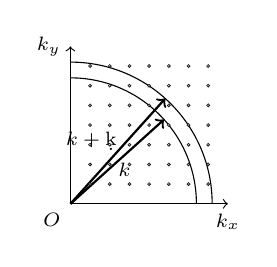
\begin{tikzpicture}[scale = .5, font = \scriptsize]
  \draw [<->] (0,4) node [left] {$k_y$} -- (0,0)
                    node [below left] {$O$} -- (4,0) node [below] {$k_x$};
  \draw (3.2,0) arc (0:90:3.2) (3.6,0) arc (0:90:3.6);
  \draw [thick, ->] (0,0) -- node [inner sep = 0pt, below right]
    {$k$} (42:3.2);
  \draw [thick, ->] (0,0) -- node [inner sep = 0pt, above left]
    {$k + \d k$} (48:3.6);
  \foreach \j in {1, ..., 7} \foreach \i in {1, ..., 7}
    \shade [shift = {(.5*\i, .5*\j)}, ball color = black]
      (0,0) circle (.05);
\end{tikzpicture}
\end{wrapstuff}
\begin{problem}[Density of States in 2D system]
  Consider free electron in a 2D box with a width of $a$.
  The allowed wave-numbers $k_x$ and $k_y$ for $x$ and $y$ directions
  respectively are expressed as $\frac{\pi n_x}a$ and $\frac{\pi n_y}{a}$,
  where $n_x$, $n_y = 1$, $2$, $3$, $\ldots$ are integer numbers.
  The following figure shows the schematic view of the 2D array of
  allowed quantum states in $k$-space.
  \wrapstuffclear
  \begin{enumext}[label = (\alph*)]
    \item Determine the area in $k$-space occupied by 1 allowed $k$ point.
    \item Express number of allowed states in the area enclosed
    by the first quarter circles with the radus of $k$ and $k + \d k$,
    where $k \gg \d k$ (Consider the spin degeneracy).
    \item Express density of allowed states in real space per unit energy.
  \end{enumext}
\end{problem}
\begin{solution}\leavevmode
  \begin{enumext}[label = (\alph*)]
    \item The area is
    $\Delta\bm k = \Delta k_x \cdot \Delta k_y = \ab(\frac\pi a)^2$.
    \item Two electrons can occupy each site
    \[
      \d N = 2 \times \frac{\d A}{\Delta \bm k}
    = \frac{\frac14[\pi(k + \Delta k)^2 - \pi k^2]}{(\pi/a)^2}
    \approx \frac{a^2k}{\pi}\d k.
    \]
    with $\ket|\uparrow>$ and $\ket|\downarrow>$.
    \item Substituting into the definition of DOS
    \[
      \text{DOS} = \frac{\d N}{\Delta A \d E}
      \xlongequal{E = \hbar^2k^2/2m} \frac{\odv N/k}{\Delta A \odv E/k}
    = \frac{m}{\pi \hbar^2}.
    \]
  \end{enumext}
\end{solution}

\begin{problem}[Density of states from a general formula]\leavevmode
  \begin{enumext}[label = (\alph*)]
    \item In a 3D solid and starting from the general formula
    \[
      g(E) = \frac{2V}{(2\pi)^3} \iint \frac{\d S_E}{|\nabla_kE|}.
    \]
    Find the expression for the electronic density of states:
    \begin{enumerate*}[label = (\roman*)]
      \item for free electrons;
      \item for electrons that obey the isotropic dispersion relation:
      $E = -E_0 - 2\gamma \cos\ab(\frac{ka}{2})$, where $E_0$, $\gamma > 0$.
    \end{enumerate*}
    \item After having established the corresponding expression for 2D,
    find $g(E)$ for (i) and (ii) above.
    \item Same question for 1D.
  \end{enumext}
\end{problem}
\begin{solution}
  In 3D, 2D, and 1D situations, the DOS are
  \begin{align*}
    g_\text{3D}(E) & = \frac{2V}{(2\pi)^3} \cdot \frac{4\pi k^2}{\nabla_kE}
  = \begin{cases}
      \frac{mV}{\pi^2\hbar^3}\sqrt{2mE},\\
      \frac{8V}{\pi^2a^3} \frac{\ab[\arccos\ab(\frac{E + E_0}{2\gamma})]}
        {\sqrt{4\gamma^2 - (E + E_0)^2}}.
    \end{cases}\\
    g_\text{2D}(E) & = \frac{2A}{(2\pi)^2} \cdot \frac{2\pi k}{\nabla_kE}
  = \begin{cases}
      \frac{mA}{\pi\hbar^2} = \text{Const},\\
      \frac{4A}{\pi a^2} \frac{\arccos\ab(-\frac{E+E_0}{2\gamma})}
        {\sqrt{4\gamma^2 - \ab(E + E_0)^2}}.
    \end{cases}\\
    g_\text{1D}(E) & = \frac{2L}{2\pi} \cdot \frac{2}{\odv E/k}
  = \begin{cases}
      \frac L{\pi\hbar} \sqrt{\frac{2m}{E}},\\
      \frac{4L}{\pi a} \frac{1}{\sqrt{4\gamma^2 - \ab(E + E_0)^2}}.
    \end{cases}
  \end{align*}
\end{solution}
\newweek
% !TeX root = ../main.tex

\section{Phonon}

\begin{problem}[Normal modes of a square lattice]
  Consider a square lattice of atoms of mass $M$,
  in which the nearest neighbors are coupled to each other
  by springs with constants $K$.
  Derive the equation of motion for the mode in which
  atomic displacements are normal to the crystal plane and
  find the dispersion of this mode.
  Analyze the behavior of this mode in the continuum limit.
\end{problem}
\begin{solution}[By TA]
  Only consider the vibration perpendicular to the surface
  \[
    M\odv[2]{U_{n,m}}t = -k \sum [u_{n,m} - u_{n\pm1,m\pm1}]
  \]
  Substitute the plane wave
  \[
    u_{n,m}(t) = U\upe^{\iu(q_xna + q_yna - \omega t)}
  \]
  we have
  \[
    -M\omega^2 = 2k[\cos(q_xa) + \cos(q_ya) - 2]
  \]
  For $|q_xa|$, $|q_ya| \ll q$, $\sin qa = qa$.
\end{solution}
\begin{solution}
  Assume the lattice constant $a$, then the lattice sites become
  \[
    \bm R_{n,m} = (na,ma), \quad n, m \in \mathbb Z.
  \]
  We consider every atom has a single degree of freedom: the out-of-plane scalar displacement $u_{n,m}(t)$. So, the spring connecting site $(n,m)$ and a neighbour $(n',m')$ has extension $\Delta = u_{n',m'} - u_{n,m}$, which brings the force to atom $(n,m)$
  \[
    F_{n,m} = -K(u_{n,m} - u_{n',m'})
  \]
  due to Hooke's law. Since every atom has four nearest neighbours:
  $(n \pm 1, m)$, $(n, m \pm 1)$, which bring four forces to the ``central atom''.
  Summing these forces
  \[
    F_{n,m}^\text{tot} = -\sum_{\braket<n,m;n',m'>} K(u_{n,m} - u_{n',m'})
  = -K(4u_{n,m} - u_{n+1,m} - u_{n-1,m} - u_{n,m+1} - u_{n,m-1})
  \]
  According to Newton's second law, we obtain the EOM
  \[
    M\ddot u_{n,m} = -K(4u_{n,m} - u_{n+1,m} - u_{n-1,m} - u_{n,m+1} - u_{n,m-1}).
  \]
  Assume the EOM has a plane-wave solution
  \[
    u_{n,m}(t) = A\upe^{\iu(k_xna+k_yma-\omega t)},
  \]
  then substitute it into the EOM, the LHS is
  \[
    \text{LHS} = M(-\omega^2)u_{n,m}
  \]
  and the RHS is
  \[
    \text{RHS} = -K(4 - \upe^{\iu k_xa} - \upe^{-\iu k_xa}
                      - \upe^{\iu k_ya} - \upe^{-\iu k_ya}) u_{n,m}
  = -2K[2 - \cos(k_xa) - \cos(k_ya)] u_{n,m}
  \]
  Finally we have the dispersion of this model
  \[
    \omega^2(\bm k) = \frac{2K}{M}[2 - \cos(k_xa) - \cos(k_ya)],\quad
    \omega(\bm k) = 2\sqrt{\frac KM} \sqrt{\sin^2\ab(\frac{k_xa}2) + \sin^2\ab(\frac{k_ya}2)}.
  \]
  In the continuum limit, i.e., $|\bm k|a \ll 1$,
  then the dispersion of this model becomes linear to $|\bm k|$
  \[
    \omega(\bm k) \approxeq
    2\sqrt{\frac KM} \sqrt{\ab(\frac{k_xa}2)^2 + \ab(\frac{k_ya}2)^2}
  = c|\bm k|
  \]
  where $c = a\sqrt{K/M}$.
\end{solution}

\clearpage

\begin{problem}[Localized phonons on an impurity]
  Consider a linear chain of identical atoms of mass $m$ each equidistant by $a$.
  \begin{enumext}[label = (\alph*)]
    \item Limiting the problem to interactions between nearest neighbors characterized by the force constant $\beta$, give the dispersion relation of longitudinal phonons and derive the expression of their group velocity.
    Express the results as a function of ``$a$'' and of the velocity of sound, $v_s$.
    What is maximum frequency of atomic vibration, $\omega_M$, when $v_s = \qty{5000}{\m/\s}$?
    \item An atom in the middle of the chain is replaced by the atom of an impurity with a mass $m'$ (where $m' < m$).
    Write the displacement equations, $u_0$, for this impurity atom and the displacement ``$u_n$'' for an atom located at a distance ``$na$''.
    Assume that the force constant $\beta$ between nearesst neighbors is the same regardless of the atom considered.
    \item The impurity atom being lighter than the others has an oscillation frequency $\omega_m'$ larger than $\omega_M$ and it drags the other neighbor atoms by its motion. We try to describe its effect with the expression of a damped wave of form: $u_n = u_0\upe^{-\alpha|x|} \upe^{\iu(\omega't-kx)}$.
    What is the value of the frequency $\omega_M'$, which is compatible with the equations of motion when the wave vector is near the boundary of the first Brillouin Zone? Verify that when $m = m'$, the solution matches that obtained in (a).
    \item After having numerically evaluated $\omega_M'$ and a when $m' = m/2$,
    sketch the instantaneous position of atoms as a function of $x$.
  \end{enumext}
\end{problem}
\begin{solution}[By TA]
  $v_y = \odv mk$.
  $v_s$ is long-wave limit $v_s$: $\lim_{k\to0}v_g = a\sqrt{\frac\beta m}$,
  and $\omega_m = \frac{2v_s}{a}$.
  \[
    u_n = u_0\upe^{-\alpha na}\upe^{\iu(\omega't - kna)}
  \]
  Substitute it into the EOM
  \[
    \begin{cases}
      -\omega'^2m' = \beta[\upe^{ax}(\upe^{\iu ka} + \upe^{-\iu ka}) - 2]\\
      -\omega'^2m = \beta[\upe^{(\alpha + \iu k)a} + \upe^{-(\alpha + \iu k)a} - 2]
    \end{cases}
  \]
  where $ka = \pi$, $\omega' = \omega_m'$,
  \[
    u_n = u_0(-1)^n \upe^{\iu\omega t} \upe^{-\alpha a|n|}
  \]
  \[
    \begin{cases}
      m\omega_m'^2 = 2\beta(1 + \upe^{-\alpha a}),\\
      m\omega'm^2 = \Delta\beta \cosh^2\ab(\frac{\alpha a}{2})
    \end{cases}
  \]
\end{solution}
\begin{solution}\leavevmode
  \begin{enumext}[label = (\alph*)]
    \item Assume the nearest-neighbor spring constant $\beta$.
    The EOM for the $n$-th atom is
    \[
      m\ddot u_n = -\beta(u_n - u_{n+1}) - \beta(u_n - u_{n-1})
    = \beta(u_{n+1} - u_{n-1} - 2u_n).
    \]
    We assume the EOM has a plane-wave solution
    $u_n(t) = A\upe^{\iu(kna-\omega t)}$, then substitute it into the EOM
    \[  
      -m\omega^2u_n = -\beta(2 - \upe^{\iu ka} - \upe^{-\iu ka})u_n
    = -\beta(2 - 2\cos(ka))u_n = -4\beta\sin^2\ab(\frac{ka}{2}),
    \]
    we have the dispersion
    \[
      \omega = 2\sqrt{\frac\beta m}\ab|\sin\ab(\frac{ka}{2})|.
    \]
    The group velocity and the velocity of sound are
    \[
      v_g(k) = \odv\omega k = a\sqrt{\frac\beta m} \cos\ab(\frac{ka}{2}),
      \qq{and}
      v_s(a) = \lim_{k\to0} v_g(k) = a\sqrt{\frac\beta m}
    \]
    then the group velocity, as well as the frequency can be expressed as
    \[
      v_g(k) = v_s \cos\ab(\frac{ka}{2}), \qq{and}
      \omega = \frac{2v_s}a \ab|\sin\ab(\frac{ka}{2})|.
    \]
    when $k = \pi/a$, the frequency arrives at a maximal value
    \[
      \omega_M = \frac{2v_s}{a} \xlongequal{v_s = \qty{5000}{\m/\s}}
      \frac{10000}{a} \unit{\s^{-1}}.
    \]
    \item The impurity is located at site $n = 0$, with mass $m'$;
    while its neighbors $n = \pm1$ with mass $m$.
    The EOM for the impurity and other atoms are
    \begin{align*}
      m'\ddot u_0 & = -\beta(u_1 - u_0) + \beta(u_{-1} - u_0)
    = \beta(u_1 + u_{-1} - 2u_0)\\
      m\ddot u_n & = \beta(u_{n+1} + u_{n-1} - 2u_n)
    \end{align*}
    \item In (a), near the boundary of the first BZ, i.e. $k = \pi/a$,
    the frequency is $\omega_\text I = 2\sqrt{\beta/m}$.
    Write the given wave form in terms of site number $n$
    \[
      u_n = A \upe^{-\alpha|n|a} \upe^{\iu(\omega't - kna)}
    \]
    Substitute it into the two EOMs in (b), and let $n = 1$
    \begin{align*}
      -\omega^2m'u_0 & = \beta(\upe^{-\alpha a-\iu ka} + \upe^{-\alpha a+\iu ka} - 2)u_0 \xlongequal{k = \pi/a} -2\beta(\upe^{-\alpha a} + 1) u_0\\
      -\omega^2m u_1 & = \beta(u_2 + u_0 - 2u_1) = \beta(\upe^{-\alpha a-\iu ka} + \upe^{\alpha a+\iu ka} - 2)u_1 \xlongequal{k = \pi/a}
      -2\beta(\cosh(\alpha a) + 1) u_1
    \end{align*}
    Derive the two expressions, we have
    \[
      \frac{m'}{m} = \frac{\upe^{-\alpha a} + 1}{\cosh(\alpha a) + 1}
    = \frac2{\upe^{\alpha a} + 1},
    \qq{and}
    \upe^{-\alpha a} + 1 = \frac{2m}{2m - m'}
    \]
    Substitute it into one of the EOM, we obtain the dispersion
    \[
      \omega_M'^2 = \omega'^2 = \frac{4\beta m}{m'(2m - m')}
    \]
    where $\omega_M'^2 = \omega'^2$ is due to the boundary of the first BZ ($k = \pi/a$).
    When $m' = m$, the frequency becomes
    \[
      \omega_M'^2 = \frac{4\beta}{m}, \qq{and} \omega_M' = 2\sqrt{\frac\beta m}
    = \omega_\text I
    \]
    which matchs that obtained in (a).
    \item Substitute $m' = m/2$ in the result of (c), we have
    $\omega_M'^2 = \frac{16}{3}\frac\beta m$.
    To simplify, we choose the time $t = 0$. Near the first BZ,
    the displacement of atoms is
    \[
      u_n = (-1)^n A\upe^{-\alpha|n|a}
    \]
    The plotted figure of atoms is attached as follows (Just show the relative position for reference).
    \begin{center}
      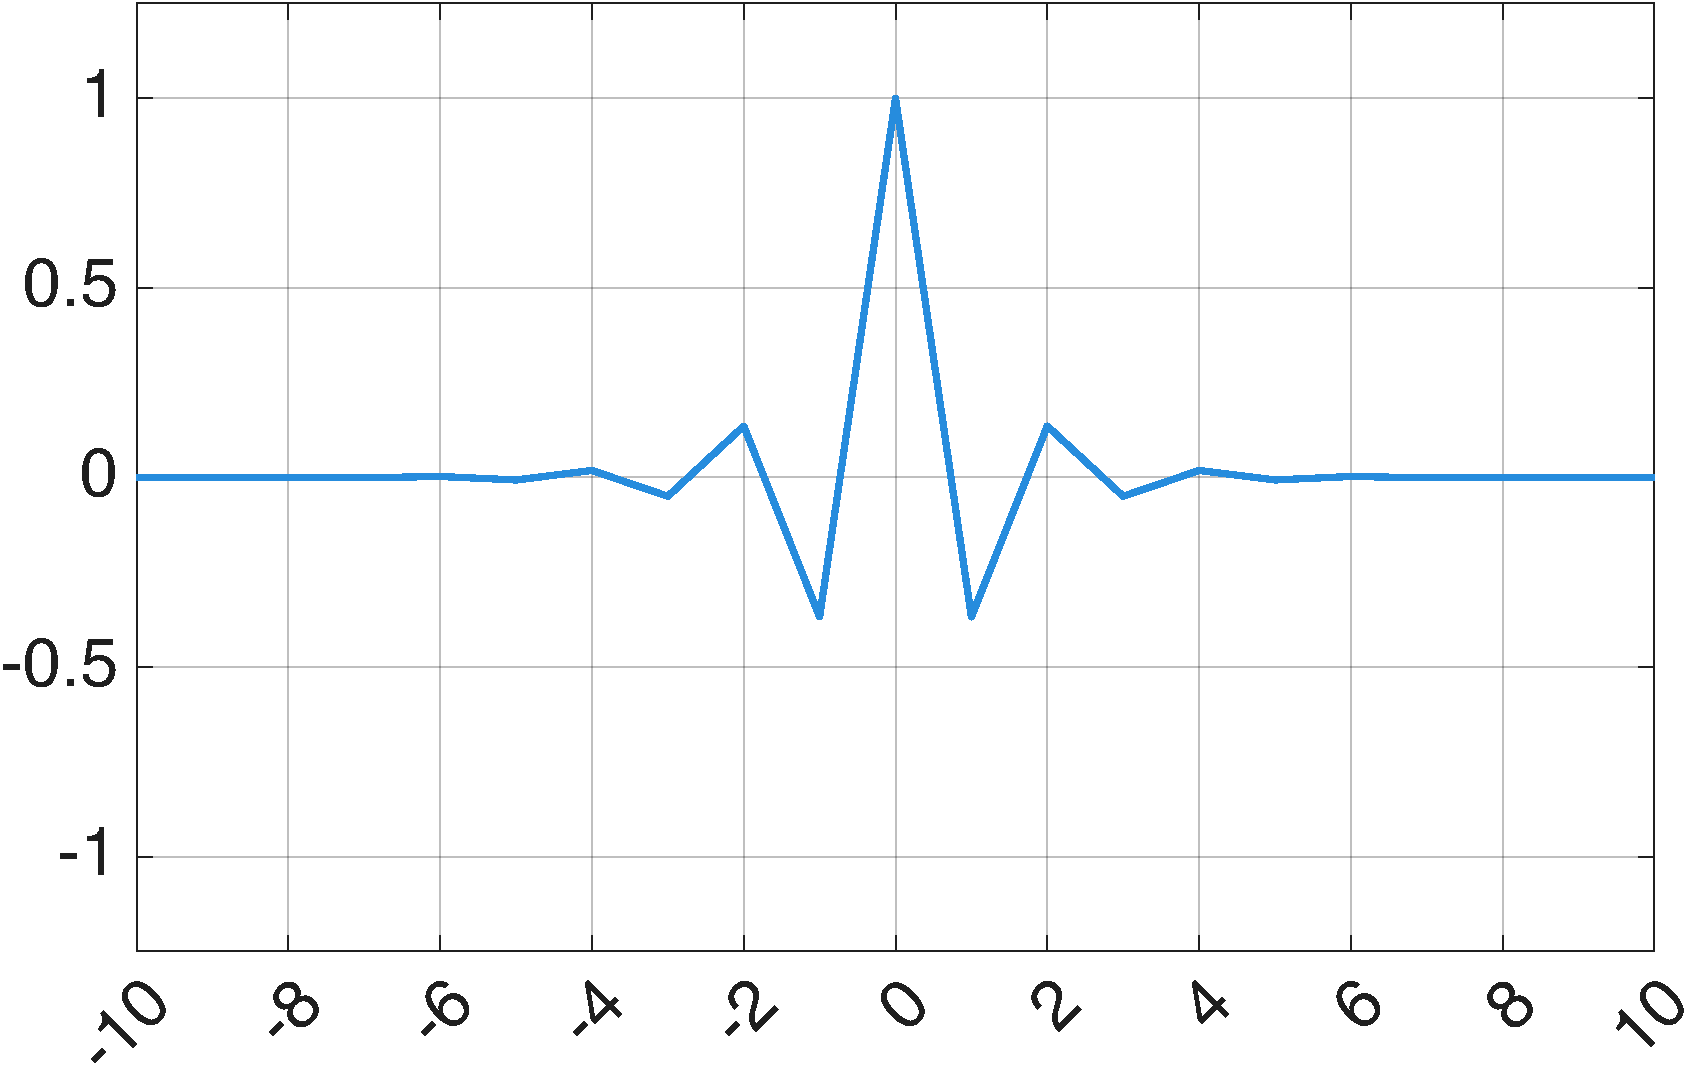
\includegraphics[width = .5\linewidth]{./media/hw2_fig.pdf}
    \end{center}
  \end{enumext}
\end{solution}

\clearpage

\begin{problem}[Density of states and specific heat of a monoatomic 1D lattice]
  Consider a row of $N$ identical atoms of mass $m$ and equidistant by $a$.
  \begin{enumext}[label = (\alph*)]
    \item Limiting the problem to interactions between nearest neighbors with a force constant $\beta$, find the expression for the dispersion relation of acoustic longitudinal vibrations propagating along this row. What is the maximum frequency $\omega_M$ of atomic vibrations, written in terms of $v_s$ and $a$? Compare the value obtained with that of $\omega_D$ deduced from the Debye model.
    \item Find the corresponding expression for the density of states $g(\omega)$.
    \item Write the expressions for internal energy $U$ and for the heat capacity $C_v$. Find the limits as these functions approach high temperatures ($\hbar\omega_M \ll k_BT$).
    \item What is the evolution of $C_v$ at low temperature? Compare the result obtained here with that deduced from the Debye model.
  \end{enumext}
\end{problem}
\begin{solution}[By TA]
  \begin{enumext}
    \item $\omega = v_sk$, $\int_0^{\omega_0} g_D(\omega) \d\omega = N$,
    $\omega(k) = 2\sqrt{\beta/m}|\sin(ka/2)|$.
    \[
      g_D(\omega) = \frac{L}{\pi} \odv k\omega = \frac L\pi \cdot \frac1{v_s}
    = \frac{Na}{\pi v_s}
    \]
    $\omega_D = \pi v_s/a$, $\omega_M = 2v_s/a$.
    \item $\braket<n> = \frac{1}{\upe^{\hbar\omega/k_BT} - 1}$,
    $\braket<E> = \braket<n>\hbar\omega$, $u_0 = \frac12\hbar\omega$.
    \[
      U = \int_0^{\omega_M} g(\omega) \ab[\frac12\hbar\omega + \frac{\hbar\omega}{\upe^{\hbar\omega/k_BT} - 1}] \d\omega
    \]
    $D_v = \odv UT$, for $\hbar\omega \ll k_BT$,
    the exponential is $\frac{\hbar\omega}{k_BT}$,
    \[
      C_v = k_B\int_0^{\omega_a} g(\omega) \d\omega = Nk_B
    \]
    \item Only $\omega \to 0$ contributes to the integration.
    \[
      \upe^{\hbar\omega/k_BT}
      \begin{cases}
        \hbar\omega \gg k_BT\frac{\hbar\omega}{\upe^{\hbar\omega k_BT}-1}
      = \hbar\omega\upe^{-\hbar\omega/k_BT},\\
        \hbar\omega \ll k_BT \upe^{\hbar\omega/k_BT} \approx k_BT
      \end{cases}
    \]
    $\omega \to 0$, $g(\omega) = g(0) = \frac{2N}{\pi\omega_M}$.
  \end{enumext}
\end{solution}
\begin{solution}\leavevmode
  \begin{enumext}[label = (\alph*)]
    \item The same to Problem 2.2(a): the dispersion
    \[
      \omega(k) = 2\sqrt{\frac\beta m}\ab|\sin\ab(\frac{ka}{2})|, ~
      v_s = \lim_{k\to0}\odv\omega k = a\sqrt{\frac\beta m}, \qq{and}
      \omega_M \xlongequal{k=\pi/a} 2\sqrt{\frac\beta m} = \frac{2v_s}{a},
    \]
    and the Debye frequency for 1D chain is $\omega_D = v_s k = \frac{\pi v_s}{a}$.
    Since $\omega_M/\omega_D = 2/\pi < 1$,
    the maximum frequency in the real dispersion is smaller than in the Debye model.
    \item In 1D chain, the number of states within $\d k$ is $2 \cdot \frac{L}{2\pi} \d k$. So, the density of states is
    \[
      g(\omega) = \frac L\pi \odv k\omega
    = \frac{2L}{\pi a\omega_M} \frac1{\sqrt{1 - (\omega/\omega_M)^2}}
    \xlongequal{L = Na} \frac{2N}{\pi\omega_M}
    \frac1{\sqrt{1 - (\omega/\omega_M)^2}}.
    \]
    \item The phonon thermal occupation
    \[
      n(\omega) = \ab[\exp\ab(\frac{\hbar\omega}{k_BT}) - 1]^{-1}
    \]
    Then the internal energy is
    \[
      U(T) = \int_0^{\omega_M} \hbar n(\omega) g(\omega) \d\omega
    = \int_0^{\omega_M} \frac{\hbar\omega}{\upe^{\frac{\hbar\omega}{k_BT}} - 1} g(\omega) \d\omega.
    \]
    and the heat capacity
    \[
      C_V(T) = \odv UT = \int_0^{\omega_M} \pdv{n(\omega)}T g(\omega) \d\omega
    \]
    At high-temperature limit, i.e., $\hbar\omega_M \ll k_BT$. The expression of internal energy and heat capacity become
    \[
      U(T) = \int_0^{\omega_M} k_BT g(\omega) \d\omega = Nk_BT,~
      C_V(T) = Nk_B.
    \]
    where applied the total number of vibration modes
    $\int_0^{\omega_M} g(\omega) \d\omega = N$.
    \newpage
    \item At low temperature limit, only small $k$ matters, i.e., the main contributions come from small $\omega$. Then, $g(\omega) = \frac L{\pi v_s}$.
    The internal energy becomes
    \[
      U = \frac L{\pi v_s} \int_0^\infty \frac{\hbar\omega}{\upe^{\frac{\hbar\omega}{k_BT}} - 1} \d\omega = \frac{\pi L(k_BT)^2}{6\hbar v_s}
    \]
    and the capacity
    \[
      C_v = \odv UT = \frac{\pi Nak_B^2T}{3\hbar v_s} \propto T
    \]
    the same conclusion as the Debye model.
  \end{enumext}
\end{solution}
\newweek
% !TeX root = ../main.tex

\paragraph{Homework \#3 Crystal lattice}

\begin{problem}[Crystallographic restriction theorem]
  Proof the crystallographic restriction theorem: Consider a crystal (i.e. with
  translational symmetry) in three dimensions that is invariant under rotations
  by an angle $2\pi/n$ around an axis. Then the only allowed possibilities are
  $n = 1$, $2$, $3$, $4$, $6$ with the case $n = 1$ being the trivial case
  with no rotational symmetry.
\end{problem}
\begin{solution}\begin{proof}
  When taking the rotation matrix to an arbitary vector
  $\bm l = (l_1, l_2, l_3)\tran$, it should leave the lattice invariant,
  the trace of the rotation matrix
  \[
    \mathbf R = \begin{pmatrix}
      \cos\theta & -\sin\theta & 0\\
      \sin\theta & \cos\theta & 0\\
      0 & 0 & 1
    \end{pmatrix}
  \]
  must be integers, then $\Tr(\mathbf R) \in \mathbb Z$,
  $n \in \{1,2,3,4,6\}$.
\end{proof}
\end{solution}

\begin{wrapstuff}[r, width = .24\linewidth]
  \centering
  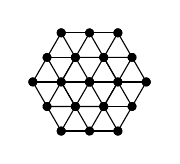
\begin{tikzpicture}[scale = .36]
    \foreach \i in {0, 1, 2, 3, 4, 5} {
      \foreach \j in {0, 1, 2} {
        \draw [rotate around = {-\i * 60:(0,0)}]
          ({-2 + \j/2}, {sqrt(3)*\j/2}) --++ (2,0);
          \foreach \k in {0, 1, 2}
            \fill [rotate around = {-\i * 60:(0,0)}]
              ({-\j + \k/2}, {sqrt(3)*\k/2}) circle (.16);
      }
      \draw [rotate around = {-\i * 60:(0,0)}] (-1,0) --++ (1,{sqrt(3)});
    }
  \end{tikzpicture}
\end{wrapstuff}
\begin{problem}[2D triangular lattice]
  Let us consider a two-dimen\-sional triangular lattice as shown in the
  following figure.
  \wrapstuffclear
  \begin{enumext}
    \item Identify the primitive unit cell of the two-dimensional triangular
    lattice. Find the basis vectors.
    \item Construct the basis vectors of the reciprocal unit cell.
  \end{enumext}
\end{problem}
\begin{solution}\leavevmode
  \begin{enumext}
    \item $\bm a_1 = a(1,0)$, $\bm a_2 = a \ab(\frac12, \frac{\sqrt3}{2})$.
    \item Using the relation $\bm a_i \cdot \bm b_j = 2\pi\delta_{ij}$ for
    $\bm a_{1,2}$ and $\bm b_{1,2}$, then
    $\bm b_1 = \frac{2\pi}a \ab(1, -\frac1{\sqrt3})$,
    $\bm b_2 = \frac{2\pi}a \ab(0, \frac2{\sqrt3})$.
  \end{enumext}
\end{solution}

\begin{problem}[Properties of the reciprocal lattice]\leavevmode
  \begin{enumext}
    \item Show that all reciprocal lattice vectors of the form
    $\bm G = h\bm A + k\bm B + l\bm C$ are perpendicular to the planes of the
    same indices $(h, k, l)$ in real space.
    \item Show that the distance $d_{h,k,l}$ between two consecutive planes
    $(h, k, l)$ is inversely proportional to $|\bm G_{h,k,l}|$.
    \item Find $d_{h,k,l}$ for a simple cubic lattice and an orthorhombic
    lattice ($a \neq b \neq c$, $\alpha = \beta = \gamma = \pi/2$).
  \end{enumext}
\end{problem}
\begin{solution}\leavevmode
  \begin{enumext}
    \item
    \begin{proof}
      Express $\bm G$ in terms of the reciprocal lattice vectors
      \[
        \bm G = \frac{2\pi}{\bm a_1 \cdot (\bm a_2 \times \bm a_3)}
           [h(\bm a_2 \times \bm a_3) + k(\bm a_3 \times \bm a_1)
          + l(\bm a_1 \times \bm a_2)]
      \]
      with the Miller indices $h:k:l = \frac1{a_1}:\frac1{a_2}:\frac1{a_3}$.
      In real space, the normal vector of the plane $(h, k, l)$ can be
      expressed as\\
      \begin{minipage}{.64\linewidth}
        \[
          \begin{aligned}
            \hat{\bm n}_{hkl} & \sim \bm r_1 \times \bm r_2
          = \frac1{hkl} [h(\bm a_2 \times \bm a_3) \\
        & \quad + k(\bm a_3 \times \bm a_1) +
                  l(\bm a_1 \times \bm a_2)],\\
          \bm r_1 & = \vec{DE} = \bm a_2/k - \bm a_1/h,\\
          \bm r_2 & = \vec{EF} = \bm a_3/l - \bm a_2/k.
          \end{aligned}
        \]
      \end{minipage}
      \hfill
      \begin{minipage}{.32\linewidth}
        \centering
        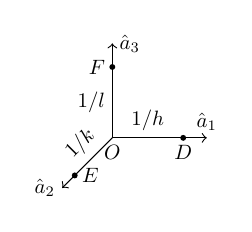
\begin{tikzpicture}[scale = .75, every node/.style = {scale = .75}]
          \draw [->] (0,0) -- (1.6,0) node [above] {$\hat a_1$};
          \draw [->] (0,0) -- (0,1.6) node [right] {$\hat a_3$};
          \draw [->] (0,0) -- (-135:1.2) node [left] {$\hat a_2$};
          \fill (1.2,0) circle (.05) node [below] {$D$};
          \node [above] at (.6,0) {$1/h$};
          \fill (0,1.2) circle (.05) node [left] {$F$};
          \node [left] at (0,.6) {$1/l$};
          \fill (-135:.9) circle (.05) node [right] {$E$};
          \node [above left, inner sep = -3pt] at
            (-135:.45) {\rotatebox{45}{$1/k$}};
          \node [below] at (0,0) {$O$};
        \end{tikzpicture}
      \end{minipage}
      Hence, $\hat{\bm n}_{hkl} \parallel \bm G$, so $\bm G$ is perpendicular
      to $(h, k, l)$ plane.
    \end{proof}
    \item \begin{proof}
    The vectors pointing to the $n + 1$ and $n$-th plane satisfy
    \[
      \bm G \cdot \bm d_{n+1} = 2\pi(n + 1), \qq{and}
      \bm G \cdot \bm d_n = 2\pi n,
    \]
    where $\bm d_{n+1} - \bm d_n = d \hat{\bm n}$. Combine the two relations
    \[
      \bm G \cdot(\bm r_{n+1} - \bm r_n) = \bm G \cdot \bm{\hat n} d = 2\pi d.
    \]
    So, we proved $d = 2\pi/(\bm G_{h,k,l} \cdot \bm{\hat n})
    = 2\pi/|\bm G_{h,k,l}|$.
    \end{proof}
    \item For a simple cubic lattice
    \[
      \bm a = (a,0,0), \quad \bm b = (0,b,0), \quad \bm c = (0,0,c).
    \]
    Then, the reciprocal vectors can be expressed as
    \[
      \bm G = \frac{2\pi h}{a} \bm{\hat x} +
              \frac{2\pi k}{b} \bm{\hat y} +
              \frac{2\pi l}{c} \bm{\hat z}.
    \]
    So, we obtain the distance $d = \frac{2\pi}{|\bm G|}
    = \ab(\frac{h^2}{a^2} + \frac{k^2}{b^2} + \frac{l^2}{c^2})^{-1/2}$.
  \end{enumext}
\end{solution}

\begin{problem}[Atomic planes and Miller indices: application to lithium]
  The Bravais lattice of lithium is simple cubic with lattice parameter
  $a = \qty{3.48}\angstrom$.
  \begin{enumext}
    \item Suppose that the atoms (assumed to be spheres) are placed along the
    $[111]$, represent the atomic distribution along the following faces
    $(100)$, $(110)$, $(111)$, and $(201)$.
    \item For each such 2D structure, state the direction and basis vector,
    $\bm a$ and $\bm b$ of the elementary lattice as well as the value of the
    angle, $\gamma$.
    \item Find the atomic concentration and the mass density of lithium
    ($A \approx 7$).
  \end{enumext}
\end{problem}
\begin{solution}\leavevmode
  \begin{enumext}
    \item (b)
    \begin{enumext}
      \item [$(100)$] $\bm a = (0,a,0)$, $\bm b = (0,0,a)$,
      $\gamma = \braket<a,b> = \qty{90}\degree$.
      \item [$(110)$] $\bm a = (a,-a,0)$, $\bm b = (0,0,a)$,
      $\gamma = \braket<a,b> = \qty{90}\degree$.
      \item [$(111)$] $\bm a = (a,0,-a)$, $\bm b = (0,a,a)$,
      $\gamma = \braket<a,b> = \qty{60}\degree$.
      \item [$(201)$] $\bm a = (0,a,0)$, $\bm b = (a,0,-2a)$,
      $\gamma = \braket<a,b> = \qty{90}\degree$.
    \end{enumext}
    \addtocounter{enumXi}{1}
    \item Since the atoms are placed along the $[111]$, then every cubic
    lattice's corners has an atom, i.e., it is equivalent that there is an
    atom in every lattice. So, the atomic concentration is
    \[
      n = \frac1V = \frac1{a^3} = \qty{2.3728e28}{atoms/\m^3}.
    \]
    The mass density is
    \[
      \rho = n m_\text{atom} = nA/N_A = \qty{275.816}{\kg/\m^3}.
    \]
  \end{enumext}
\end{solution}
\newweek
% !TeX root = ../main.tex

\section{X-ray diffraction}

\begin{problem}[Structure factor for a tri-atomic basis]
  Consider a linear crystal with lattice constant $a$ in which the basis
  consists of atom of species $A$ at $0$ and two atoms of species $B$ at $1/3$
  and $2/3$.
  \begin{enumext}
    \item Find the structure factor of such a crystal.
    \item X-rays of wavelength $\lambda (= a/4)$ irradiate this crystal at an
    oblique incidence ($\qty{45}\degree$). Using the Ewald construction in the
    plane of incidence, show graphically, the diffraction directions and
    indicate the relative weights of the different diffracted intensities.
    \item State the physical significance of the vector $\bm k$ from which the
    extremity is on a plane passing through the origin of the reciprocal lattice.
  \end{enumext}
\end{problem}
\begin{solution}[By TA]
  \begin{enumext}
    \item \[
      S_a = \sum_j f_j \upe^{-\iu \bm a \cdot \bm r_j}
    = f_A \upe^{-\iu\bm G\cdot0} + f_B(\upe^{-\iu\bm G\cdot\frac a3\hat x}
    + \upe^{-\iu\bm a\cdot\frac23 a\hat x})
    = f_A + 2f_B\cos(\frac{2\pi}{3}h)
    = \begin{cases}
      f_A + 2f_B,\\
      f_A - f_B
    \end{cases}
    \]
    \item $k = \frac{2\pi}{\lambda} = \frac{8\pi}{a}$,
    \[
      k\cos\qty{45}\degree - k\cos\theta = G_x
    \]
    $\cos\theta = \frac{h + 2\sqrt2}{4} \in [-1, 1]$.
  \end{enumext}
\end{solution}
\begin{solution}\leavevmode
  \begin{enumext}
    \item Substitute $r_i = 0$, $\frac a3$, $\frac{2a}3$ into the definition of
    the structure factor
    \begin{align*}
    S(h) & = f_A\upe^{\iu G\cdot 0} + f_B\upe^{\iu G\cdot\frac a3}
           + f_B\upe^{\iu G\cdot\frac{2a}{3}}
      \xlongequal{G = 2\pi h/a} f_A + f_B
             \ab(\upe^{\iu\frac{2\pi h}{3}} + \upe^{\iu\frac{4\pi h}{3}})\\
    & \xlongequal{\text{Euler's formula}}
    \begin{cases}
      f_A + 2f_B, & h = 3n\\
      f_A - f_B,  & \text{otherwise}
    \end{cases}
    \end{align*}
    \item The wave number
    \[
      k = \frac{2\pi}{\lambda} = \frac{8\pi}{a} = 4b_0,
    \]
    where $b_0 = \frac{2\pi}{a}$ is the reciprocal lattice vector.
    The incident wavevector is
    \[
      \bm k_i = \ab(k/\sqrt2, -k/\sqrt 2)
    \]
    \begin{paracol}{2}
    Then, the Ewald circle satisfies
    \[
      \ab(x + k/\sqrt2)^2 + \ab(y - k/\sqrt2)^2 = k^2
    \]
    and we can obtain the two intersection on $x$-axis: $x_1 = 0$ and
    $x_1 = -\sqrt2k$.

    Obviously, $x_1 = 0b_0$, $n_1 = 0$;
    $x_2 = -5.656b_0$, $n_2 = -5.656$.
    \switchcolumn \centering
    \vspace*\fill
    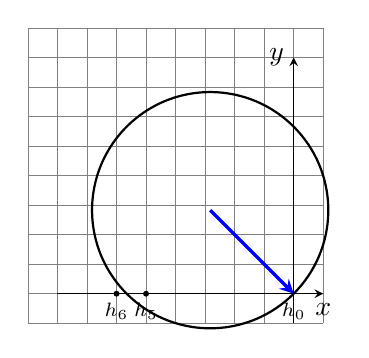
\begin{tikzpicture}[scale = .75]
      \draw [help lines, step = .5cm] (-4.5,4.5) grid (.5,-.5);
      \draw [-stealth] (-4,0) -- (.5,0) node [below] {$x$};
      \draw [-stealth] (0,-.5) -- (0,4) node [left] {$y$};
      \draw [thick] ({-2/sqrt(2)}, {2/sqrt(2)}) circle (2);
      \draw [blue, very thick, -stealth] ({-2/sqrt(2)}, {2/sqrt(2)}) -- (0,0);
      \fill (-2.5,0) circle (.05) (-3,0) circle (.05);
      \node [below] at (0,0) {$\scriptstyle h_0$};
      \node [below] at (-2.5,0) {$\scriptstyle h_5$};
      \node [below] at (-3,0) {$\scriptstyle h_6$};
    \end{tikzpicture}
    \vspace*\fill
    \end{paracol}
    Since $n$ is not an integer, no other reciprocal lattice points lies on the
    Ewald circle except the one on the original point.
    The intensity of each diffraction order is proportional to $|S(h)|^2$, i.e.,
    \[
      I_h \propto |S(h)|^2 =
      \begin{cases}
        (f_A + 2f_B)^2, & h = 3m,\\
        (f_A - f_B)^2,  & \text{otherwise}
      \end{cases}
    \]
    \item The tip of $\bm k$ lying on a plane through the origin of the
    reciprocal lattice means the Bragg condition is satisfied for diffraction.
  \end{enumext}
\end{solution}

\begin{problem}
  The main experimental methods of X-ray diffraction are
  \begin{enumext*}[label = (\alph*), columns = 2]
    \item the Laue method
    \item the crystal rotation method
    \item(2) the powder method (or the Debye-Scherrer method)
  \end{enumext*}
  Describe the corresponding experimental set-up and with the help of the Ewald
  construction in reciprocal space, deduce the observed diffraction patterns in
  each case.
\end{problem}
\begin{solution}\leavevmode
  \begin{enumext}
    \item Laue Method
    \begin{enumext}
      \item Setup: Stationary single crystal, polychromatic X-rays.
      \item Ewald \& Pattern: A continuous range of Ewald sphere radii (due to
      varying $\lambda$) means many reciprocal lattice points lie on some
      sphere. This produces a pattern of sharp spots, each from a different
      $(hkl)$ plane and wavelength. The spot arrangement directly reveals the
      crystal's symmetry.
    \end{enumext}
    \item Crystal Rotation Method
    \begin{enumext}
      \item Setup: Rotating single crystal, monochromatic X-rays.
      \item Ewald \& Pattern: The fixed Ewald sphere is intersected by rotating
      reciprocal lattice points. This generates discrete spots or arcs on the
      detector. Measuring the rotation angles and intensities of these spots
      allows for the determination of the unit cell and atomic structure.
    \end{enumext}
    \item Powder Method
    \begin{enumext}
      \item Setup: Powdered sample (random crystallites), monochromatic X-rays.
      \item Ewald \& Pattern: Each set of $(hkl)$ planes forms a spherical shell
      in reciprocal space. The Ewald sphere's intersection with these shells
      creates cones of diffracted beams (Debye cones), which appear as
      characteristic rings on the detector. The ring positions
      ($2\theta$ angles) provide $d$-spacings for phase identification and
      lattice parameter calculation.
    \end{enumext}
  \end{enumext}
\end{solution}
\newweek
% !TeX root = ../main.tex

\paragraph{Homework \#5 Nearly free electron model}

\begin{problem}[Compare Kronig-Penney model with the nearly free electron model]
  The Kronig-Penney model allows one to consider both the nearly-free-electron
  and tight-binding limits. Consider the (repulsive) Dirac-Kronig-Penney model.
  It gives the following implicit equation for the energy bands
  \[
    \cos(ka) = \cos(qa) + u\sin(qa)/qa,
  \]
  where $q = \sqrt{2mE}/\hbar$ and $u = \frac{mU_0a}{\hbar^2} > 0$. Assuming
  that $u \ll q$, find the solution of above equation near the Bragg points
  $k \approx \pm\frac\pi a$, $\pm\frac{2\pi}{a}$, $\ldots\,$. Compare your
  result with that of the nearly-free electron model. (Reminder: the $\approx$
  sign means that $k$ is close yet no equal to the wavenumber of the Bragg
  point.)
\end{problem}
\begin{solution}
  Near the Bragg points, assume
  \[
    ka = n\pi + \kappa a, \qq{and}
    qa = q_n a + \delta.
  \]
  with $|\kappa|$, $|\delta| \ll 1$, $q_n = n\pi/a$.
  Keep the 2nd order of $\kappa$ and $\delta$, the implict equation can be
  written as
  \[
    (-1)^n \ab[1 - \frac12(\kappa a)^2] = (-1)^n \ab(1 - \frac12\delta^2)
                                        + u\frac{(-1)^n\delta}{n\pi}.
  \]
  Then, we can have the solution of $\delta$
  \[
    \delta = u/n\pi \pm \sqrt{(u/n\pi)^2 + (\kappa a)^2}.
  \]
  Since $q = \sqrt{2mE}/\hbar$, then we have
  \[
    E = \hbar^2(q_n + \delta/a)^2/2m
      \approxeq E_n^0 + \hbar^2 q_n \delta/ma,
  \]
  where $E_n^0 = \frac{\hbar^2q_n^2}{2m}$.
  Substitute $q_n = n\pi/a$, and the solution of $\delta$ into the expression
  of $E$
  \[
    E = E_n^0 + \frac{n\pi\hbar^2\delta}{m}
  = E_n^0 + \frac{n\pi\hbar^2}{ma^2}
            \ab[\frac{u}{n\pi} \pm
            \sqrt{\ab(\frac{u}{n\pi})^2 + (\kappa a)^2}].
  \]
  Substitute $u = mU_0a/\hbar^2$ into the expression above
  \[
    E = E_n^0 + \frac{U_0}{a} \pm
        \sqrt{\ab(\frac{U_0}{a})^2 + \ab(\frac{n\pi\hbar^2\kappa}{ma})^2}
  \]
  with the band gap
  \[
    \Delta E_n = E_+ - E_-
  = 2\sqrt{\ab(\frac{U_0}{a})^2 + \ab(\frac{n\pi\hbar^2\kappa}{ma})^2}.
  \]
  When $\kappa a \to 0$, the energy band and the band gap become
  \[
    E = E_n^0 + U_0/a \pm U_0/a, \qq{and} \Delta E_n = 2U_0/a.
  \]
  The results perfectly match that of the nearly-free electron model.
\end{solution}

\begin{problem}[Nearly free electron model]
  Consider 2D electrons subject to a weak periodic potential
  \[
    U(x,y) = U_0 [\cos(2\pi x/a) + \cos(2\pi y/a)].
  \]
  \begin{enumext}
    \item Find the energy bands near the \emph{edges} of the first Brillouin
    zone. (Hint: the edges of the Brillouin zone are the Bragg planes where the
    eigenstates are doubly degenerate.) Plot the bands and isoenergetic
    surfaces.
    \item Repeat the analysis of part (a) for regions near the \emph{corners}
    of the first Brillouin zone, where there are four degenerate eigenstates.
  \end{enumext}
\end{problem}
\begin{solution}\leavevmode
  \begin{enumext}
    \item The reciprocal vectors are
    $\bm G_1 = \ab(\frac{2\pi}{a}, 0)$,
    $\bm G_2 = \ab(0, \frac{2\pi}{a})$.
    Apply Fourier transformation to the potential
    \[
      U(x,y) = \frac{U_0}{2}
      \ab[e^{\pm\iu\bm G_1 \cdot \bm r} + e^{\pm\iu\bm G_2 \cdot \bm r}]
      = \sum_G U_G \upe^{\iu\bm G \cdot \bm r}.
    \]
    So, the Fourier coefficient is $U_{\pm G_{1,2}} = U_0/2$.
    Near the zone edge (e.g., $k_x = \pi/a$), consider a wavevector
    \[
      \bm k = (\pi/a + q_x,  k_y)
    \]
    with $|q_x| \ll \pi/a$. The two nearly degenerate plane waves are
    $\ket|\bm k>$ and $\ket|\bm k - \bm G_1>$.
    Their free-electron energies are
    \begin{multline*}
      E^{(0)}(\bm k, \bm k - \bm G_1)
    = \frac{\hbar^2}{2m} \ab[\ab(\pm\frac{\pi}{a} + q_x)^2 + k_y^2]\\
    \approx E_0 \pm \alpha q_x
    = \frac{\hbar^2}{2m} \ab[\ab(\frac{\pi}{a})^2 + k_y^2]
      \pm \frac{\hbar^2 \pi}{m a} q_x.
    \end{multline*}
    The perturbation couples these states with matrix element
    $\braket<\bm k|U|\bm k - \bm G_1> = U_0/2$.
    In the subspace $\{\ket|\bm k>, \ket|\bm k - \bm G_1>\}$, the Hamiltonian is
    \[
      H = \begin{pNiceMatrix}[first-col, first-row]
                      & \ket|\bm k>      & \ket|\bm k - \bm G_1>\\
          \bra<\bm k| & E_0 + \alpha q_x & U_0/2 \\
\bra<\bm k - \bm G_1| & U_0/2 & E_0 - \alpha q_x
      \end{pNiceMatrix}.
    \]
    From the eigenfunction $\det(\mathcal H - E\identity) = 0$,
    one can obtain the eigenvalues
    \[
      E_{\pm} = E_0 + \frac{\hbar^2 q_x^2}{2m}
        \pm \sqrt{\ab(\frac{\hbar^2 \pi}{m a} q_x)^2 + \ab(\frac{U_0}{2})^2}.
    \]
    \item The corners ($M$-point) of the first Brillouin zone are
    \begin{align*}
      \bm k_1 & = \bm k_0 = (+\pi/a, +\pi/a), \\
      \bm k_2 & = \bm k_0 - \bm G_1 = (-\pi/a, +\pi/a), \\
      \bm k_3 & = \bm k_0 - \bm G_2 = (+\pi/a, -\pi/a), \\
      \bm k_4 & = \bm k_0 - \bm G_1 - \bm G_2 = (-\pi/a, -\pi/a),
    \end{align*}
    with the same free-electron energies
    \[
      E_0 = \frac{\hbar^2}{2m} \ab(k_x^2 + k_y^2) = \frac{\hbar^2 \pi^2}{m a^2}.
    \]
    In the basis
    $\{\ket|\bm k_1>, \ket|\bm k_2>, \ket|\bm k_3>, \ket|\bm k_4> \}$,
    states are coupled if they differ by $\pm \bm G_1$ or $\pm \bm G_2$.
    The non-zero off-diagonal matrix elements are
    \[
      \braket<\bm k_1|U|\bm k_2> = \braket<\bm k_1|U|\bm k_3> =
      \braket<\bm k_2|U|\bm k_4> = \braket<\bm k_3|U|\bm k_4> = \tfrac{U_0}2.
    \]
    The Hamiltonian is
    \[
      \mathcal H = E_0 \identity + \frac{U_0}{2}
      \begin{pNiceMatrix}[first-col, first-row]
      & \ket|\bm k_1> & \ket|\bm k_2>
      & \ket|\bm k_3> & \ket|\bm k_4> \\
        \bra<\bm k_1| & 0 & 1 & 1 & 0 \\
        \bra<\bm k_2| & 1 & 0 & 0 & 1 \\
        \bra<\bm k_3| & 1 & 0 & 0 & 1 \\
        \bra<\bm k_4| & 0 & 1 & 1 & 0
      \end{pNiceMatrix}.
    \]
    From the eigenfunction $\det(\mathcal H - E\identity) = 0$, one can obtain
    the eigenvalues $E = \{E_0 + U_0,\ E_0 - U_0,\ E_0,\ E_0\}$.
  \end{enumext}
\end{solution}
\newweek
% !TeX root = ../main.tex

\section{Tight binding model}

\begin{problem}[Tight bindings in the BCC and FCC lattices]
  We consider identical atoms located at points of a lattice that are
  body-centered cubic (\textbf{BCC: i}) and face-centered cubic
  (\textbf{FCC: ii}).
  \begin{enumext}
    \item For each case, determine the dispersion relation for $s$-electrons,
    having the general form
    \[
      E = -\alpha - \gamma \sum_s \upe^{-\iu \bm k \cdot \bm R_s},
    \]
    where $\alpha$ and $\gamma$ are the positive energies that can be calculated
    and $\mathbf R_s$ represents the vectors that connect an atom located at the
    origin to each of its nearest neighbors.
    \item Find the expressions for $E$ at the points located at the intersection
    of the first Brillouin zone with the directions $[100]$, $[110]$,
    and $[111]$ and thus the value $E(\Gamma)$ to the center of this zone.
    \item Deduce the total width of the corresponding band, $\Delta E$, and find
    the expression for the effective mass $m^*$ in the vicinity of $\Gamma$ as
    well as the shape of constant energy surfaces around this point.
  \end{enumext}
\end{problem}
\begin{solution}[By TA]
  $\frac a2(\pm1,\pm1,\pm1)$
  \[
    \sum_s\upe^{-\iu \bm k\cdot \bm R_s}
  = \sum_{u,v,w} \ab[-\frac a2\iu(uk_x + vk_y + wk_z)]
  = 8\cos\ab(\frac{ak_x}2) \cos\ab(\frac{ak_y}2) \cos\ab(\frac{ak_z}2)
  \]
  $\frac a2(\pm 1,0,\pm 1)$, $\frac a2(\pm1,\pm1,0)$, $\frac a2(0,\pm1,\pm1)$.

  For BCC $E(\Gamma) = E(0,0,0) = -\alpha - 8\gamma$.
  \[
    |\bm k|^2 = |\bm k - \bm G|^2
  = |\bm k|^2 - 2\bm k \cdot \bm G + |\bm G|^2, \quad
  2\bm k \cdot \bm G = |\bm G|^2
  \]
  The nearest $\frac{2\pi}{a}(\pm1,0,\pm1)$
  \[
    \begin{cases}
      k_x \pm k_y = \pm\frac{2\pi}{a},\quad
      k_y \pm k_z = \pm\frac{2\pi}{a},\quad
      k_z \pm k_x = \pm\frac{2\pi}{a}.
    \end{cases}
  \]
  For $[1,0,0]$
  \[
    \begin{cases}
      k_x = t, \\
      k_y = k_z = 0
    \end{cases}
  \]
  $(\pm\frac{2\pi}{a}, 0, 0)$, $E = -\alpha + 8\gamma$.
  For $[1,1,0]$
  \[
    \begin{cases}
      k_x = k_y = t,\\
      k_z = 0
    \end{cases}
  \]
  $(\frac\pi a, \frac\pi a, 0)$, $E = -\alpha$.
  For $[1,1,1]$: $k_x = k_y = k_z = t$,
  $(\frac\pi a, \frac\pi a, \frac\pi a)$, $E = -\alpha$.

  For FCC:
  \[
    E(\Gamma) = -\alpha - 12\gamma
  \]
  Consider the nearest $\frac{2\pi}{a}(\pm 1, \pm 1, \pm 1)$.
  \[
    \bm k \cdot \bm a = \ab(\frac{2\pi}{a})^2 \cdot \frac32,
  \]
  \[
    \pm k_x\pm k_y\pm k_z = \frac{3\pi}{a}
  \]
  Sub-nearest: $\frac{2\pi}{a}(\pm2,0,0)$,
  \[
    k_x = \pm\frac{2\pi}{a}, \quad
    k_y = \pm\frac{2\pi}{a}, \quad
    k_z = \pm\frac{2\pi}{a}.
  \]
  For $[1,0,0]$: $(\frac{2\pi}{a},0,0)$
  \[
    \begin{cases}
      k_x = t,\\
      k_y = k_z = 0
    \end{cases},\quad
    E = -\alpha + 4r
  \]
  For $[1,1,0]$: $(\frac{3\pi}{2a}, \frac{3\pi}{2a}, 0)$
  \[
    \begin{cases}
      k_x = k_y = t,\\
      k_z = 0
    \end{cases}, \quad
    E = -\alpha - 2\gamma + 4\sqrt2r
  \]
  For $[1,1,1]$: $(\frac\pi a, \frac\pi a, \frac\pi a)$
  \[
    k_x = k_y = k_z = t, \quad E = -\alpha
  \]
  \[
    E_k = E_0 + \frac{\hbar^2}{2m} (\bm k - \bm k_0)^2 \qq{for $k \to 0$}
  \]
  Use some approximation
  \[
    k \to 0, \quad
    \cos\frac{ak}{2} = 1 - \frac{a^2k^2}{8}
  \]
  BCC:
  \[
    E_k = -\alpha - 8\gamma \ab(1 - \frac{a^2k_x^2}{8})\ab( ...k_y) \ab( ... k_z)
  = -\alpha - 8\gamma + \gamma a^2k^2
  \]
  where $\gamma a^2 = \frac{\hbar^2}{2m^*}$, $m^* = \frac{\hbar^2}{2\gamma a}$.
  
\end{solution}
\begin{solution}[$\text{i} = \text{BCC}$, $\text{ii} = \text{FCC}$]
  Assume the lattice constant $a$.
  \newcounter{case} \setcounter{case}{1}
  \begin{enumext}[label = (\alph*\textsubscript{\roman{case}})]
    \item Each atom has 8 NNs, i.e.,
    \[
      \{\bm R_s\} = \ab\{\frac a2(\pm1, \pm1, \pm1)\}
    \]
    Then, the sum in the general form becomes
    \[
      \sum_s \upe^{-\iu \bm k \cdot \bm R_s}
    = \sum_{\sigma_x=\pm} \sum_{\sigma_y=\pm} \sum_{\sigma_z=\pm}
      \upe^{-\iu\frac a2\sigma_xk_x} \cdot
      \upe^{-\iu\frac a2\sigma_yk_y} \cdot
      \upe^{-\iu\frac a2\sigma_zk_z}
    = 8\cos\ab(\frac{ak_x}2) \cos\ab(\frac{ak_y}2) \cos\ab(\frac{ak_z}2)
    \]
    Hence, the dispersion relation is
    \[
      E(\bm k) = -\alpha - 8\gamma
      \cos\ab(\frac{ak_x}2) \cos\ab(\frac{ak_y}2) \cos\ab(\frac{ak_z}2)
    \]
    \item \begin{enumext}[columns = 2]
      \item $\Gamma$ point: $\bm k = (0,0,0)$,
      $E(\Gamma) = -\alpha - 8\gamma$.
      \item $[100]$: $\bm k = \frac{2\pi}{a}(1, 0, 0)$,
      $E(X) = -\alpha + 8\gamma$.
      \item $[110]$: $\bm k = \frac{2\pi}{a}(\frac12, \frac12, 0)$,
      $E(N) = -\alpha$.
      \item $[111]$: $\bm k = \frac\pi a(1, 1, 1)$,
      $E(P) = -\alpha$
    \end{enumext}
    \item The $\cos$ terms in the general form differs between
    $[-8\gamma, +8\gamma]$. So, the energy gap is
    \[
      \Delta E_\text{BCC} = (-\alpha + 8\gamma) - (-\alpha - 8\gamma)
    = 16\gamma
    \]
    The dispersion relation can be expanded around the $\Gamma$ point
    \[
      E(\bm k) = -\alpha - 8\gamma\ab[1
        - \frac12\ab(\frac{ak_x}{2})^2
        - \frac12\ab(\frac{ak_y}{2})^2
        - \frac12\ab(\frac{ak_z}{2})^2 ]
    \xlongequal{k^2=k_x^2+k_y^2+k_z^2} -\alpha - 8\gamma + \gamma a^2 k^2
    \]
    Then, the effective mass $m^* = \frac{\hbar^2}{\pdv[2]E/k}
    = \frac{\hbar^2}{2\gamma a^2}$.
    \addtocounter{case}{1} \setcounter{enumXi}{0}
    \item Each atom has 12 NNs, i.e.,
    \[
      \{\bm R_s\} = \ab\{
        \frac a2(\pm1, \pm1, 0),
        \frac a2(\pm1, 0, \pm1),
        \frac a2(0, \pm1, \pm1).
      \}
    \]
    Then, the sum in the general form becomes
    \begin{align*}
      \sum_s \upe^{-\iu \bm k \cdot \bm R_s} &
    = \sum_{\text{cyclic}(x,y,z)} \sum_\pm
      \upe^{-\iu\frac a2(\pm k_i\pm k_j)} \\ &
    = 4\ab[
        \cos\ab(\frac{ak_x}2) \cos\ab(\frac{ak_y}2) +
        \cos\ab(\frac{ak_y}2) \cos\ab(\frac{ak_z}2) +
        \cos\ab(\frac{ak_z}2) \cos\ab(\frac{ak_x}2) ]
    \end{align*}
    Hence, the dispersion relation is
    \[
      E(\bm k) = -\alpha - 4\gamma \ab[
        \cos\ab(\frac{ak_x}2) \cos\ab(\frac{ak_y}2) +
        \cos\ab(\frac{ak_y}2) \cos\ab(\frac{ak_z}2) +
        \cos\ab(\frac{ak_z}2) \cos\ab(\frac{ak_x}2) ]
    \]
    \item \begin{enumext*}[columns = 2, label = \roman*.]
      \item $\Gamma$ point: $\bm k = (0,0,0)$,
      $E(\Gamma) = -\alpha - 8\gamma$.
      \item $[100]$: $\bm k = \frac{2\pi}{a}(1, 0, 0)$,
      $E(X) = -\alpha - 4\gamma$.
      \item(2) $[110]$ point: $\bm k = \frac{2\pi}{a}(\frac34, \frac34, 0)$,
      $E(N) = -\alpha + \gamma(4\sqrt2 - 2)$.
      \item(2) $[111]$ point: $\bm k = \frac\pi a(1, 1, 1)$,
      $E(P) = -\alpha - 12\gamma$
    \end{enumext*}
    \item The $\cos$ terms in the general form differs between
    $[-12\gamma, +4\gamma]$. So, the energy gap is
    \[
      \Delta E_\text{FCC} = (-\alpha + 4\gamma) - (-\alpha - 12\gamma)
    = 16\gamma
    \]
    The dispersion relation can be expanded around the $\Gamma$ point
    \begin{align*}
      E(\bm k) & = -\alpha - 4\gamma\sum_{\text{cyclic}(x,y,z)}\ab[1
        - \frac12\ab(\frac{ak_i}{2})^2
        - \frac12\ab(\frac{ak_j}{2})^2 ]\\ &
    = -\alpha - 12\gamma + 4\gamma\ab[
        \ab(\frac{k_xa}2)^2 + \ab(\frac{k_ya}2)^2 + \ab(\frac{k_za}2)^2]
    = -\alpha - 12\gamma + \gamma a^2k^2
    \end{align*}
    Then, the effective mass $m^* = \frac{\hbar^2}{\pdv[2]E/k}
    = \frac{\hbar^2}{2\gamma a^2}$.
  \end{enumext}
\end{solution}
\newweek
% !TeX root = ../main.tex

\section{Semiconductor}

\begin{problem}[Elementary study of an intrinsic semiconductor]
  \begin{paracol}{2}
    Consider a semiconductor characterized by a constant density of states
    ($g(E) = C$) in both the valence and conduction band. These bands,
    separated by $E_g$, have a respective width of $E_V$ and $E_C$
    (see the Figure).
    \begin{enumext}
      \item Knowing that the Fermi level $E_F$ is in the bandgap
      ($5k_BT < E_F < E_g - 5k_BT$), leading to the conventional simplification
      for $f(E)$ (The Boltzmann approximation can be applied), find the
      expression for the number of electrons $n$ in the conduction band and the
      number of holes $h$ in the valence band respectively as a function of the
      data and absolute temperature.
    \end{enumext}
    \switchcolumn \centering
    \begin{tikzpicture}
      \draw [->] (0,0) node [left] {$0$} -- (3,0) node [right] {$g(E)$};
      \draw [->] (0,-2.8) -- (0,3.5) node [right] {$E$};
      \draw (0,-2.5) node [left] {$-E_V$} -- (1,-2.5) -- (1,0)
       node [above] {$C$};
      \draw (0,1) node [left] {$E_g$} -- (1,1) -- (1,3) -- (0,3)
       node [left] {$E_C + E_g$};
      \draw (0,.5) node [left] {$E_F$} --++ (.2,0);
    \end{tikzpicture}
  \end{paracol}
  \begin{enumext}[topsep = 0pt]
    \setcounter{enumXi}{1}
    \item Deduce the expression for the volumetric density of intrinsic
    carriers $n_i$ at ambient temperature ($k_BT = \qty{25}\meV$) as well as
    the position of the Fermi level $E_{F_i}$.

    Numerical applications: $E_g = \qty{0.7}\eV$, $E_C = E_V = \qty5\eV$,
    and $C = \qty{2e21}{electrons/\cm^3/\eV}$.
    \item At the same temperature, what is the intrinsic electronic
    conductivity of this material? Take
    $\mu_h = \mu_e = \qty{1000}{\cm^2/\V\s}$.
    \item The material is doped with $N_0$ boron impurities. Find the
    expressions and the new values of $n_d$, $h_d$, $\sigma_d$, and $E_{F_d}$
    with $N_0 = \num{e12}$ impurities per $\unit{\cm^3}$ and next with
    $N_0 = \num{e14}$ impurities per $\unit{\cm^3}$.
  \end{enumext}
\end{problem}
\begin{solution}\leavevmode
  \begin{enumext}
    \item The number of electrons in the conduction band
    \[
      n = \int_{E_g}^{E_g+E_c} g(E) f(E) \d E
        = Ck_BT\upe^{-\frac{(E_g-E_F)}{k_BT}}(1 - \upe^{-\frac{E_C}{k_BT}})
        \xlongequal[\text{Boltzmann approximation}]{E_C\gg k_BT}
          Ck_BT\upe^{-\frac{E_g-E_F}{k_BT}}.
    \]
    The number of electrons in the valence band
    \[
      h = \int_{-E_V}^0 g(E) [1 - f(E)] \d E
        \approxeq Ck_BT\upe^{-\frac{E_F}{k_BT}} (1 - \upe^{-\frac{E_V}{k_BT}})
        \xlongequal[\text{Boltzmann approximation}]{E_V\gg k_BT}
          Ck_BT\upe^{-\frac{E_F}{k_BT}}.
    \]
    where $f(E) \approxeq \upe^{-\frac{E-E_F}{k_BT}}$,
          $[1 - f(E)] \approxeq \upe^{\frac{E-E_F}{k_BT}}$.
    \item For the intrinsic carriers, the number of electrons and holes are the
    same
    \[
      n = Ck_BT\upe^{-\frac{E_g-E_F}{k_BT}} =
      h = Ck_BT\upe^{-\frac{E_F}{k_BT}}, \quad
      E_g - E_F = E_F.
    \]
    Then, the Fermi level is at mid-gap, i.e., $E_F = \frac{E_g}{2}$.
    Substitute it back into the expression of $n$ (or $h$),
    we get the intrinsic carrier concentration
    \[
      n_i = Ck_BT\upe^{-\frac{E_g}{2k_BT}}.
    \]
    Apply the parameters, $n_i = \qty{4.158e19}{\m^{-3}}$,
    $E_F = \qty{0.35}\eV$.
    \item The conductivity
    \[
      \sigma_i = e(n_i\mu_e + n_i\mu_h) = \qty{1.332}{\siemens/\m}.
    \]
    \item Boron is an acceptor, so doping concentration $N_A = N_0$.
    Now, the number of electrons and holes
    \[
      n = n_i,\ h = n_i \longrightarrow
      n_d = n,\ h_d = n + N_0,
    \]
    and they satisfy the identity: mass-action law
    \[
      n_i^2 = n_dh_d = n(n + N_0).
    \]
    We can solve that
    \[
      n = \frac{\sqrt{N_0^2 + 4n_i^2} - N_0}2,\quad
      n_d = n = \frac{\sqrt{N_0^2 + 4n_i^2} - N_0}2,\quad
      h = n + N_0 = \frac{\sqrt{N_0^2 + 4n_i^2} + N_0}2.
    \]
    The conductivity becomes
    \[
      \sigma_d = e(n_d\mu_e + h_d\mu_h).
    \]
    From $h = Ck_BT\upe^{-\frac{E_F}{k_BT}}$, we can obtain the Fermi level
    \[
      E_{F_d} = k_BT \ln\frac{C k_BT}{h_d}.
    \]
    Apply the parameters (with the previous $n_i = \qty{4.158e19}{\m^{-3}}$)
    \begin{enumext}[columns = 2]
      \item $N_0 = \qty{e18}{\m^{-3}}$.\\
      The numbers of the acceptors and donators
      \begin{gather*}
        n_d = \qty{4.108e19}{\m^{-3}},\\
        h_d = \qty{4.208e19}{\m^{-3}}.
      \end{gather*}
      The conductivity and the Fermi level
      \[
        \sigma_d = \qty{1.332}{\siemens/\m},~
        E_{F_d} = \qty{0.350}\eV.
      \]
      \item $N_0 = \qty{e20}{\m^{-3}}$.\\
      The numbers of the acceptors and donators
      \begin{gather*}
        n_d = \qty{1.503e19}{\m^{-3}},\\
        h_d = \qty{1.150e20}{\m^{-3}}.
      \end{gather*}
      The conductivity and the Fermi level
      \[
        \sigma_d = \qty{2.083}{\siemens/\m},~
        E_{F_d} = \qty{0.325}\eV.
      \]
    \end{enumext}
  \end{enumext}
\end{solution}
\newweek
% !TeX root = ../main.tex

\section{Electrons in a magnetic field}

\begin{problem}[Onsager formula]
  Suppose that the electron spectrum for a tetragonal lattice can be described
  by the following equation
  \[
    E_k = \frac{\hbar^2 k_x^2}{2m_{xx}} + \frac{\hbar^2 k_y^2}{2m_{xx}}
        + \frac{\hbar^2 k_z^2}{2m_{zz}},
  \]
  with $m_{xx} \neq m_{zz}$. Using the Onsager formula for the cyclotron mass,
  $m_c = \frac{\hbar^2}{2\pi} \pdv A{E_k}$ with $A$ being the area of an
  isoenergetic contour perpendicular to the magnetic field. Find $m_c$ for the
  case when the magnetic field is
  \begin{enumext}[columns = 2]
    \item Along the $z$-axis.
    \item In the $x-y$ plane.
  \end{enumext}
\end{problem}
\begin{solution}\leavevmode
  \begin{enumext}
    \item For $\bm B \parallel \hat z$, the motion of electrons will
    perpendicular to $\hat z$, i.e., parallel to $x-y$ plane. The equation of
    motion becomes
    \[
      E_k = \frac{\hbar^2}{2m_{xx}}(k_x^2 + k_y^2),
    \]
    with the equation of the motion boundary in $k$-space
    \[
      k_\parallel^2 \equiv k_x^2 + k_y^2 = \frac{2m_{xx} E_k}{\hbar^2}.
    \]
    Then, we get the radius. The circle area of the isoenergetic contour is
    \[
      A = \pi k_\parallel^2 = \frac{2\pi m_{xx} E_k}{\hbar^2}.
    \]
    Substituting to the definition of cyclotron mass, we can obtain
    \[
      m_c = \frac{\hbar^2}{2\pi} \pdv A{E_k}
    = \frac{\hbar^2}{2\pi} \frac{2\pi m_{xx}}{\hbar^2} = m_{xx}.
    \]
    \item Simply taking $\bm B \parallel \hat x$, then orbits lie in the
    $k_y-k_z$ plane with an ellipse area. The equation of motion becomes
    \[
      E_k = \frac{\hbar^2 k_y^2}{2m_{xx}} + \frac{\hbar^2 k_z^2}{2m_{zz}},
    \]
    with the equation of the motion boundary in $k$-space
    \[
      \frac{k_y^2}{2m_{xx}E/\hbar^2} + \frac{k_z^2}{2m_{zz}E/\hbar^2} = 1.
    \]
    Then we get the semi-axes. The ellipse area of the isoenergetic contour is
    \[
      A = \pi \sqrt{\frac{2m_{xx}E}{\hbar^2}}
              \sqrt{\frac{2m_{zz}E}{\hbar^2}}
        = \frac{2\pi E}{\hbar^2}\sqrt{m_{xx}m_{zz}}
    \]
    Substituting to the definition of cyclotron mass, we can obtain
    \[
      m_c = \frac{\hbar^2}{2\pi} \pdv A{E_k} = \sqrt{m_{xx}m_{zz}}.
    \]
  \end{enumext}
\end{solution}

\begin{problem}[Integer Quantum Hall Effect]
  The Hall resistance $R_{xy}$ of a two-dimensional electron gas is measured as
  a function of magnetic field $B$ at a very low temperature. A series of
  plateaus are observed at values $R_{xy} = \frac{h}{(\nu e^2)}$, where $\nu$ is
  an integer. Simultaneously, the longitudinal resistance $R_{xx}$ shows peaks
  and drops to zero.
  \begin{enumext}
    \item Explain physically why $R_{xx}$ drops to zero whenever $R_{xy}$ is on
    a plateau.
    \item A sample has an electron density of $n_s = \qty{4.0e11}{\cm^{-2}}$.
    \begin{enumext}
      \item Calculate the filling factor $\nu$ at $B = \qty{2.0}\T$.
      \item What is the expected value of $R_{xy}$ on the plateau nearest to
      this field?
      \item How many Landau levels are completely filled at this plateau?
    \end{enumext}
    \item Why is the IQHE used as a resistance standard? Which two fundamental
    constants are involved?
  \end{enumext}
\end{problem}
\begin{solution}\leavevmode
  \begin{enumext}
    \item When the Hall resistance $R_{xy}$ is on a plateau, the Fermi energy
    lies in a mobility gap between Landau levels. All extended states in the
    bulk are absent, making the bulk insulating. Current flows only along
    dissipationless chiral edge states.
    
    At the edges, backscattering is prevented by spatial separation: even if
    impurities or imperfections exist along an edge, they may cause small
    forward deviations in an electron's path but cannot reverse its direction,
    so no resistance is produced. With no extended states in the bulk to allow
    dissipation and no backscattering at the edges, the longitudinal voltage
    drop vanishes, giving $R_{xx} = 0$.
    \item \begin{enumext}
      \item From the degeneracy of Landau level $n_s = \nu \frac{eB}{h}$,
      we can obtain the filling factor
      \[
        \nu = \frac{n_sh}{eB}
      = \frac{\qty{4.0e15}{\m^{-2}} \times \qty{6.626e-34}{\J\cdot\s}}
          {\qty{1.602e-19}\coulomb \times \qty{2.0}\T} = 8.271.
      \]
      \item Substituting the values into the expression of the Hall resistance
      \[
        R_{xy} = \frac{R_K}{\tilde\nu}
      = \frac{h}{\tilde\nu e^2} = \qty{3226.60}\ohm.
      \]
      where $\tilde \nu$ is the nearest integer of $\nu$.
      \item The filling factor $\tilde \nu = 8$ directly corresponds to the
      number of completely filled Landau levels.
    \end{enumext}
    \item IQHE provides a quantized Hall resistance
    \[
      R_H = \frac{h}{e^2},
    \]
    which precisely quantized and only based on two fundamental constants:
    The Planck constant $h$ and the elementary charge $e$, so it is used as
    a resistance standard.
  \end{enumext}
\end{solution}
\newpage
\begin{problem}[Lifshitz-Kosevich formula]
  The Lifshitz-Kosevich formula describes the amplitude of the Shubnikov-de Haas
  (SdH) oscillations. The amplitude $\Delta R$ is proportional to the factor:
  $R_T = \frac{\lambda(T)}{\sinh \lambda(T)}$,
  where $\lambda(T) = 2\pi^2 \frac{k_BTm^*}{\hbar eB}$.
  \begin{enumext}
    \item A researcher measures the SdH oscillation amplitude $\Delta R$ at a
    fixed magnetic field $B$ as a function of temperature $T$. How can they use
    this data to determine the effective mass $m^*$ of the charge carriers?
    \item Another researcher fixes the temperature $T$ and measures the SdH
    amplitude $\Delta R$ as a function of $1/B$. They find that the amplitude
    decreases exponentially with $1/B$. What physical parameter does this decay
    reveal, and what does a rapid decay imply about the quality of the sample?
  \end{enumext}
\end{problem}
\begin{solution}\leavevmode
  \begin{enumext}
    \item Take $\alpha = \frac{2\pi^2k_Bm^*}{\hbar eB}$,
    then $\lambda(T) = \alpha T$.
    Since at $T \gg 1$, the
    amplitude $\Delta R$ satisfies
    \[
      \Delta R \propto R_T = \frac{\alpha T}{\sinh(\alpha T)}
      \to \frac12 \alpha T \upe^{-\alpha T}, \quad
      \Delta R = \tilde C T\upe^{-\alpha T}
    \]
    Take the logarithm to the two sides
    \[
      \ln \Delta R = \ln \tilde C + \ln T - \alpha T, \quad
      \ln\ab(\frac{\Delta R}T) = -\alpha T + C,
    \]
    where $C = \ln\tilde C$.
    \begin{paracol}{2}
      So, one can take the data at high temperature,
      and use some software tool to convert the original data from
      $T$-$\Delta R$ to $T$-$\ln\ab(\frac{\Delta R}{T})$,
      then plot the new data set like the right figure.
      \switchcolumn \centering
      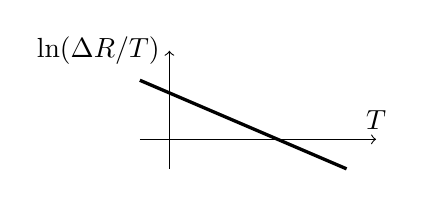
\begin{tikzpicture}[scale = .75]
        \draw [->] (-.5,0) -- (3.5,0) node [above] {$T$};
        \draw [->] (0,-.5) -- (0,1.5) node [left] {$\ln(\Delta R/T)$};
        \draw [very thick] (-.5,1) --++ (3.5,-1.5);
      \end{tikzpicture}
    \end{paracol}
    By fitting the slope $k = -\alpha$ that fits the figure, one can obtain
    the effective mass
    \[
      m^* = \frac{\alpha \hbar eB}{2\pi^2k_B}
    = -\frac{k \hbar eB}{2\pi^2k_B}
    \]
    \item Similarly to part (a), we take $T \gg 1$.
    Since $\Delta R$ is proportional to $R_TR_DR_S$, and if we only
    consider the magnetic variable $B$, then $\Delta R \propto R_TR_D$.
    To be more specific,
    \[
      \Delta R \propto \frac{2\pi^2 k_BTm^*}{\hbar e} \cdot \frac1B \cdot
               \upe^{-\frac{2\pi^2 k_BTm^*}{\hbar e} \cdot \frac1B} \cdot
               \upe^{-\frac{\pi m^*}{e\tau_q} \cdot \frac1B}
    = \tilde C \cdot \frac1B \cdot \upe^{-(\alpha+\beta/\tau_q)\cdot\frac1B}
    \]
    where the coefficients $\alpha$ and $\beta$ can be easily known since we
    have already obtained the effective mass. Taking the logarithm to both
    sides, we can obtain
    \[
      \ln(\Delta R)  = C - \ln B - \ab(\alpha + \frac\beta{\tau_q}) \frac1B,
    \]
    Since the effective mass $m^*$ has been determined from (a), so the
    coefficients $\alpha$ and $\beta$ are known, and the slope directly reveals
    the quantum scattering rate $1/\tau_q$.

    A rapid exponential decay corresponds to a short $\tau_q$, meaning a short
    mean free path and therefore significant disorder: an indicator of poor
    sample quality.
  \end{enumext}
\end{solution}
\newweek
% !TeX root = ../main.tex

\section{Band structure of graphene}

\begin{problem}
  In the calculation of the monolayer graphene band structure using
  tight-binding model, if we keep the contribution of the next-nearest
  hopping $t'$.
  \begin{enumext}
    \item Write down the dispersion relation.
    \item Expand the energy spectrum around the Dirac point up to second order.
    Search the literature and check what's trigonal warping effect is in
    a monolayer.
  \end{enumext}
\end{problem}
\begin{solution}\leavevmode
  \begin{enumext}
    \item 
  \end{enumext}
\end{solution}

\begin{problem}
  Graphene has the record room-temperature electron mobility, mainly due to two
  reasons. The first is the high Debye temperature ($\sim\qty{2100}\K$) that
  suppresses phonon scattering arising from the in-plane covalent $sp^2$ bonding
  between carbon atoms. The second one is related to its unique linear Dirac
  band, resulting in massless Dirac fermions ($m^* = 0$) near the Dirac point.
  However, if we apply the definition of the effective
  mass $m^* = \hbar^2\ab(\odv[2]{E(k)}k)^{-1}$ to the band dispersion of
  graphene $(E_\pm(k) = \pm \hbar v_Fk)$, we will get diverging $m^*$ and
  non-differentiable Dirac point. Please explain this contradiction.
\end{problem}
\begin{solution}
  The contradiction arises from applying different definitions of ``mass'' to
  graphene's unique band structure. The description of ``massless Dirac
  fermions'' comes from the analogy to relativistic particles.
  \par \vspace{.5\baselineskip}
  From a massless special relativity particle like a photon to the electrons in
  the graphene, their dispersion relations have the comparasion
  \[
    E = pc \Longrightarrow E = \pm \hbar v_F k = p v_F
  \]
  with $v_F$ playing the role of $c$. Hence, electrons near the Dirac point
  behave as if they have zero rest mass.
  \par \vspace{.5\baselineskip}
  However, the conventional effective mass $m^* = \hbar^2 (\odv[2]E/k)^{-1}$ is
  defined under the parabolic-band approximation $E \propto k^2$. For graphene's
  linear dispersion, $\odv[2]E/k = 0$ away from $k = 0$, leading
  to $m^* \to \infty$ mathematically. At $k = 0$ the dispersion is
  non-differentiable, so the formula breaks down.
  \par \vspace{.5\baselineskip}
  Physically, this infinite effective mass reflects that the electron's speed is
  constant at $v_F$: An external force parallel to its momentum cannot change
  its speed, much like a photon's speed is fixed at $c$. Thus, the ``massless''
  label refers to the relativistic analogy, while the divergent $m^*$ indicates
  the inapplicability of the parabolic effective mass concept to a linear band.
\end{solution}
\end{multicols}

\end{document}